\documentclass[prb,11pt,tightenlines,twocolumn,aps]{revtex4-1}

\usepackage{amsmath}    % need for subequations
\usepackage{graphicx}   % need for figures
\usepackage{verbatim}   % useful for program listings
\usepackage{color}      % use if color is used in text
\usepackage{subfigure}  % use for side-by-side figures
\usepackage{hyperref}   % use for hypertext links, including those to external
                        % documents and URLs 
\usepackage{blindtext}  % fill text
\usepackage[dvipsnames]{xcolor}
\usepackage{multirow}
% \usepackage{showframe}
% \usepackage[inline]{showlabels}

\raggedbottom           % don't add extra vertical space

\begin{document}

\title{Pure Spin Current Injection in Hydrogenated Graphene Structures}
\author{Reinaldo Zapata-Pe\~na\textsuperscript{1},
        Bernardo S. Mendoza\textsuperscript{1},
        Anatoli I. Shkrebtii\textsuperscript{2}}
\affiliation{\textsuperscript{1}Centro de Investigaciones en \'Optica, Le\'on,
Guanajuato 37150, M\'exico}
\affiliation{\textsuperscript{2}University of Ontario, Institute of Technology,
Oshawa, ON, L1H 7L7, Canada}

\date{\today}

\begin{abstract}
\blindtext
\end{abstract}

\maketitle

%%%%%%%%%%%%%%%%%%%%%%%%%%%%%%%%%%%%%%%%%%%%%%%%%%%%%%%%%%%%%%%%%%%%%%%%%%%%%%
%%%%%%%%%%%%%%%%%%%%%%%%%%%%%%%%%%%%%%%%%%%%%%%%%%%%%%%%%%%%%%%%%%%%%%%%%%%%%%
%%%%%%%%%%%%%%%%%%%%%%%%%%                         %%%%%%%%%%%%%%%%%%%%%%%%%%%
%%%%%%%%%%%%%%%%%%%%%%%%%% I N T R O D U C T I O N %%%%%%%%%%%%%%%%%%%%%%%%%%%
%%%%%%%%%%%%%%%%%%%%%%%%%%                         %%%%%%%%%%%%%%%%%%%%%%%%%%%
%%%%%%%%%%%%%%%%%%%%%%%%%%%%%%%%%%%%%%%%%%%%%%%%%%%%%%%%%%%%%%%%%%%%%%%%%%%%%%
%%%%%%%%%%%%%%%%%%%%%%%%%%%%%%%%%%%%%%%%%%%%%%%%%%%%%%%%%%%%%%%%%%%%%%%%%%%%%%

\section{Introduction}
\label{sec:introduction}


\begin{figure}[ht!]
    \centering
    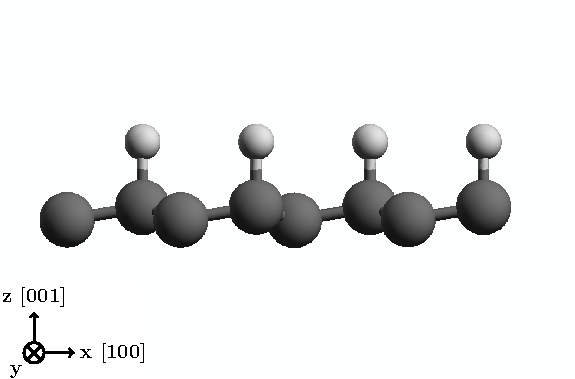
\includegraphics[width=\linewidth]{figures/upstruc2}
    \\
    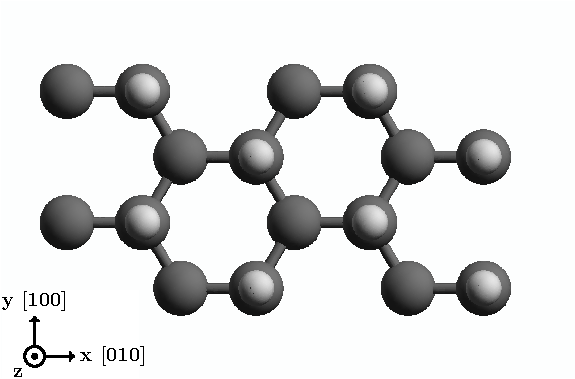
\includegraphics[width=\linewidth]{figures/upstruc1}
    \caption{Up structure}
    \label{fig:up-struc}
\end{figure}
\begin{figure}[ht!]
    \centering
    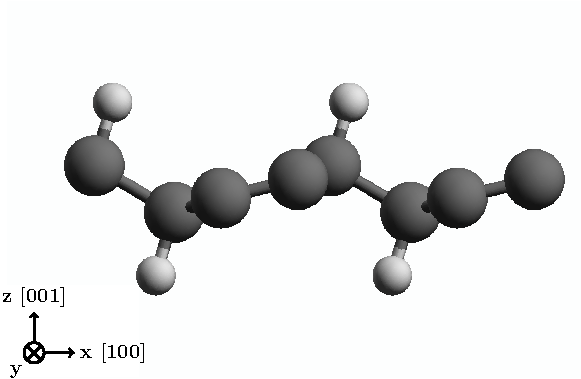
\includegraphics[width=\linewidth]{figures/altstruc2}
    \\
    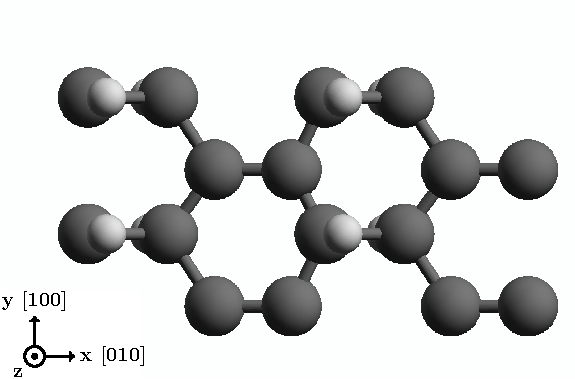
\includegraphics[width=\linewidth]{figures/altstruc1}
    \caption{Alt structure.}
    \label{fig:alt-struc}
\end{figure}


{
\color{blue}
Spintronics is an emerging research field of electronics in which the
manipulation and transport of spin of electrons in a solid state 
media plays the determining role adding a new degree of freedom to the
conventional charge manipulation.\cite{wolfSC04,fabianAPS07}
% 
At present there is an increasing interest in attain the same level of control
over the transport of spin at micro or nano scales as has been done for the
flow of charge in typical electronic devices.\cite{awschalomNP2007} Some
semiconductor spintronics devices have been proposed \cite{majumdarAPL06,
dattaAPL90} and some of them require spin polarized electrical current
\cite{awschalomSSBM13} or pure spin currents (PSC). In PSCs there is no net
motion of charge; spin-up electrons move in a given direction while spin-down
electrons travel in the opposite one. This phenomena can result from spin
injection,\cite{malPRB03} Hall Effects,\cite{sinovaPRB04} interference of two
optical beams,\cite{bhatPRL00, najmaiePRB03} or one photon absorption of
linearly polarized light\cite{bhatPRL05} and has been observed in gallium
arsenide (GaAs),\cite{zhaoPRL2006, stevensPRL03} aluminum-gallium arsenide
(AlGaAs),\cite{stevensPRL03} and Co$_2$FeSi.\cite{kimuraNGPAM12}

% Since its discovery, graphene has attracted a great interest in materials
% science and condensed matter physics being a new class of materials that are
% only one atom thick\cite{geimNM07}. 
% 
Graphene, an allotrope of carbon with hexagonal 2D lattice structure presents
properties like fractional quantum Hall effect at room temperature, excellent
thermal transport properties, high conductivity and strength \cite{geimNM07,
reinaNL08, novoselov2S07, balandinNL08} being then a perfect platform to be
used in two-dimensions electronic systems; however most electronic applications
are disabled by the absence of a semiconducting gap. Recent studies demonstrate
that the band gap of graphene can be opened by applying an electric
field,\cite{zhangN09} reducing the surface area,\cite{hanPRL07} or applying
uniaxial strain.\cite{niACSN08} Another possibility to open the gap is by
doping; this has been successfully achieved using nitrogen,\cite{weiNL2009}
boron-nitrogen,\cite{guoIJ11} silicon,\cite{colettiPRB10} noble-metals, and
hydrogen.\cite{eliasS09, guisingerNL09, samarakoonACSN10}
% 
Depending on the percentage of hydrogenation and spatial configurations of
hydrogen-carbon bonds, hydrogenated graphene can result in different spatial
configurations.
% 
In this paper we present two 50\% hydrogenated graphene non centrosymmetric
structures both presenting a discernible band gap: the \emph{up} structure,
shown in Fig. \ref{fig:up-struc}, has hydrogen atoms bonded to the carbon layer
only in the upper side of the structure while the \emph{alt} structure, shown
in Fig. \ref{fig:alt-struc}, has hydrogen alternating in the upper and bottom
sides of the carbon slab.\cite{zapataPSB2016}

Using those structures we address a theoretical study of the spin velocity
injection (SVI) by one-photon absorption of linearly polarized light that does
not seem to have been reported previously.
% 
We calculated the responses for the particular cases when the spin of electrons
is directed along the the $z$ Cartesian coordinate, perpendicular to the $xy$
plane of the structure, or for the case when the velocity is directed along the
$x$ and $y$ Cartesian direction on the $xy$ plane of the structures.
% 
The SVI ($\mathcal{V}^{\mathrm{ab}}(\omega,\alpha)$) is optical effect that
quantifies the velocity at which a PSC moves along the Cartesian direction
$\mathrm{b}$ with the spin of electron polarized along the Cartesian direction
$\mathrm{a}$. One photon absorption of linearly polarized light can promote a
distribution of electrons in $\mathbf{k}$ space regardless the symmetry of the
material resulting in a not net electrical current. Then, the electrons excited
to the conduction bands at opposite $\mathbf{k}$ points will result in opposite
spin polarizations producing no net spin injection.\cite{bhatPRL05} If the
crystalline structure of the material is not centrosymmetric the spin
polarization injected at a given $\mathbf{k}$ point could not
vanish\cite{alvaradoPRL85, schmiedeskampPRL88} and then a PSC will be produced
since the velocities of electrons at opposite $\mathbf{k}$ points are opposite.

This paper is organized as follows. In Section \ref{sec:theory} we present the
theory and formulas that describe PSC and SVI. In Section \ref{sec:results} we
describe the details of calculations and the corresponding SVI spectra for the 
\emph{up} and \emph{alt} structures. Finally, in Section 

}

%%%%%%%%%%%%%%%%%%%%%%%%%%%%%%%%%%%%%%%%%%%%%%%%%%%%%%%%%%%%%%%%%%%%%%%%%%%%%%
%%%%%%%%%%%%%%%%%%%%%%%%%%%%%%%%%%%%%%%%%%%%%%%%%%%%%%%%%%%%%%%%%%%%%%%%%%%%%%
%%%%%%%%%%%%%%%%%%%%%%%%%%%%%%%%               %%%%%%%%%%%%%%%%%%%%%%%%%%%%%%%
%%%%%%%%%%%%%%%%%%%%%%%%%%%%%%%%  T H E O R Y  %%%%%%%%%%%%%%%%%%%%%%%%%%%%%%%
%%%%%%%%%%%%%%%%%%%%%%%%%%%%%%%%               %%%%%%%%%%%%%%%%%%%%%%%%%%%%%%%
%%%%%%%%%%%%%%%%%%%%%%%%%%%%%%%%%%%%%%%%%%%%%%%%%%%%%%%%%%%%%%%%%%%%%%%%%%%%%%
%%%%%%%%%%%%%%%%%%%%%%%%%%%%%%%%%%%%%%%%%%%%%%%%%%%%%%%%%%%%%%%%%%%%%%%%%%%%%%

\section{Theory} % (fold)
\label{sec:theory}


%%%%%%%%%%%%%%%%%%%%%%%%%%%%%%%%%%%%%%%%%%%%%%%%%%%%%%%%%%%%%%%%%%%%%%%%%%%%%%
%%%%%%%%%%%%%%%%%%%%%%%%%%% Theory: Spin velocity %%%%%%%%%%%%%%%%%%%%%%%%%%%%
%%%%%%%%%%%%%%%%%%%%%%%%%%%%%%%%%%%%%%%%%%%%%%%%%%%%%%%%%%%%%%%%%%%%%%%%%%%%%%


In this section, we report a summary of the theory that involves the PSC
phenomena from which rises the SVI treated in this paper. The full description 
of it was presented by Bhat and Sipe et. al.\cite{bhatPRL05}
 
As mentioned before in Section \ref{sec:introduction}, In PSCs there is no net
motion of charge and spin-up electrons move in a given direction while spin-
down electrons travel in the opposite one. This effect can result from one
photon absorption of linearly polarized light by a semiconductor, with filled
valence bands and empty conduction bands, illuminated by light with photon
energy larger than the energy gap.
% note 1
Using i.e. a single weak continuous linearly polarized laser beam, is possible
to promote electrons in $\mathbf{k}$ space regardless the symmetry of the
system resulting in a net current equal to zero. Then, if the system presents
inversion of symmetry, electrons promoted to the conduction bands at opposite
$\mathbf{k}$ points will have opposite spin polarization resulting in a total
spin injection equal to zero. If the phenomena is produced in a
noncentrosymmetric semiconducting media the spin polarization injected at a
given $\mathbf{k}$ point can be held\cite{alvaradoPRL85}, resulting in a PSC
because the velocity of electrons at opposite $\mathbf{k}$ points are in
opposite directions.

\subsection{Spin velocity injection} % (fold)
\label{sec:theory-pure_spin_current}

We define the SVI as the velocity at which the spin, polarized along the
direction $\mathrm{a}$, propagates along the direction $\mathrm{b}$ as
\begin{equation}\label{eq:vab-w}
\mathcal{V}^{\mathrm{ab}}(\omega) \equiv
\frac{\dot{K}^{\mathrm{ab}}(\omega)}{(\hbar/2) \dot{n}(\omega)},
\end{equation}  
where the pure spin density injection current, $\dot{K}^{\mathrm{ab}}
(\omega)$, and the carrier injection rate, $\dot{n}(\omega)$, are given by
% 
\begin{equation}\label{eq:dot-kn}
\begin{aligned}
\dot{K}^{\mathrm{ab}}(\omega) 
&=
\mu^{\mathrm{abcd}}(\omega)
E^{\mathrm{c}}(\omega) E^{\mathrm{d*}}(\omega),
% \label{eq:dotk} 
\\
\dot{n}(\omega)
&=
\xi^{\mathrm{ab}}(\omega) E^{c }(\omega) E^{d*}(\omega),
% \label{eq:dotn}
\end{aligned}
\end{equation}
where the roman superscripts denote Cartesian directions, and if repeated, they
are to be summed over, the $\xi^{\mathrm{ab}}(\omega)$ are the carrier
generation rate tensor components and $\mu^{\mathrm{abcd}}(\omega)$ are the
pure spin-current pseudotensor components given by\cite{bhatPRL05}
\begin{equation*}\label{eq:mu}
\begin{aligned}
\mu^{\mathrm{abcd}}  (\omega) &
=
\frac{\pi e^{2}}{\hbar^{2}} \int 
\frac{d^{3}K}{8 \pi^{3}} \times \\
\sum_{vcc'}^{'}
\mathrm{Re} & \left[ K^{\mathrm{ab}}_{cc'} 
\left( 
r^{\mathrm{c}}_{vc'} 
r^{\mathrm{d}}_{cv } +
(c \leftrightarrow d)
\right) 
\right] \delta(\omega-\omega_{cv}),
\end{aligned}
\end{equation*}
where $K^{\mathrm{ab}}_{mn}(\mathbf{k}) =
\sum_{\ell}v^{\mathrm{a}}_{nl}(\mathbf{k}) S^{\mathrm{b}}_{lm}(\mathbf{k})$ are
the spin current matrix elements that, using time reversal invariance, satisfy
the relation $K^{\mathrm{ab}}_{nm}(\mathbf{-k}) = K^{\mathrm{ab*}}(\mathbf{k})
$. 
% 
The $'$ in the sum means that $c$ and $c'$ are quasi degenerate states and the
sum only covers these states and since $\mu^{\mathrm{abcd}}(\omega)$ is real we
have that $\mu^{\mathrm{abcd}}(\omega) = \mu^{\mathrm{abdc}}(\omega)$.
% 
Since we have 2D structures we use an incoming electric field parallel to the
surface, $\mathbf{E}^{a}(\omega) = E^{\mathrm{a}} e^{i(\alpha + \omega t)}$,
where the angle $\alpha$ corresponds to the linear polarization angle measured
positively in the counter-clockwise from the $x$ direction on the
surface of the structures.
% 
Then from Eq. \eqref{eq:dot-kn} we can rewrite the Eq. \eqref{eq:vab-w} and 
including the polarization angle dependence we have
\begin{widetext}
\begin{align}
\mathcal{V}^{\mathrm{ab}}(\omega,\alpha)
&= \frac{2}{\hbar}
\frac{\mu^{\mathrm{abxx}}(\omega)
E^{2}(\omega)\cos^{2}(\alpha) + 
\mu^{\mathrm{abyy}}(\omega)
E^{2}(\omega)\sin^{2}(\alpha) + 
2\mu^{\mathrm{abxy}}(\omega)
E^{2}(\omega)\cos(\alpha)\sin(\alpha)}
{\xi^{\mathrm{xx}}(\omega)
E^{2}(\omega)\cos^{2}(\alpha) + 
\xi^{\mathrm{yy}}(\omega)
E^{2}(\omega)\sin^{2}(\alpha)},
\nonumber \\
&= \frac{2}{\hbar}
\frac{\mu^{\mathrm{abxx}}(\omega)\cos^{2}(\alpha) + 
\mu^{\mathrm{abyy}}(\omega)\sin^{2}(\alpha) + 
\mu^{\mathrm{abxy}}(\omega)\sin(2\alpha)}
{\xi^{\mathrm{xx}}(\omega)\cos^{2}(\alpha) + 
\xi^{\mathrm{yy}}(\omega)\sin^{2}(\alpha)},
\label{eq:vab-aw}
\end{align}
\end{widetext}
% 
If the polarization angle is fixed to $\alpha = \frac{\pi}{4}$ the previous
expression can be reduced to 
\begin{equation*}\label{eq:vab-90deg}
\mathcal{V}^{\mathrm{ab}} (\omega)
= \frac{2}{\hbar}
\frac{\mu^{\mathrm{abxx}}(\omega) + \mu^{\mathrm{abyy}}(\omega) + 
2\mu^{\mathrm{abxy}}(\omega)}
{\xi^{\mathrm{xx}}(\omega) + \xi^{\mathrm{yy}}(\omega)}.
\end{equation*}
Two interesting possibilities to analyze the SVI are fixing the spin along any
of the three Cartesian coordinates and, for our cases, particularly for the
spin directed along $z$ directed perpendicularly to the surface of the
structure; or fixing the velocity along the $x$ or $y$ Cartesian coordinates on
the $xy$ plane of the structures. Also we can analyze the SVI contribution
coming from each layer of the structure. In following subsections we present
these three cases.

%%%%%%%%%%%%%%%%%%%%%%%%%%%%%%%%%%%%%%%%%%%%%%%%%%%%%%%%%%%%%%%%%%%%%%%%%%%%%%
%%%%%%%%%%%%%%%%%%%%%%%%%%%% Theory: Fixing spin %%%%%%%%%%%%%%%%%%%%%%%%%%%%%
%%%%%%%%%%%%%%%%%%%%%%%%%%%%%%%%%%%%%%%%%%%%%%%%%%%%%%%%%%%%%%%%%%%%%%%%%%%%%%

\subsection{Fixing spin}\label{sec:theory-fixspin}

Analyzing the SVI, Eq. \eqref{eq:vab-aw}, we define the magnitude of the spin
velocity with spin polarized along the $\mathrm{b}$ Cartesian coordinate as
\begin{equation}
|\mathcal{V}_{\sigma^{\mathrm{b}}}(\omega,\alpha)| 
=
\sqrt{
[\mathcal{V}^{\mathrm{xb}}(\omega,\alpha)]^{2}\ +
[\mathcal{V}^{\mathrm{yb}}(\omega,\alpha)]^{2}\ 
}, 
\label{eq:vs-mag}
\end{equation}
and the angle at which the spin velocity is directed on the $xy$ plane as
\begin{equation}
\gamma_{\mathrm{b}} (\omega,\alpha)
=
\tan^{-1} \left( \frac{\mathcal{V}^{\mathrm{yb}}(\omega,\alpha)}
{\mathcal{V}^{\mathrm{xb}}(\omega,\alpha)} \right),
\label{eq:gamma-ang}
\end{equation}
where this angle is measured in the counter-clockwise direction from the
positive $x$ Cartesian coordinate. We also define two special
angles
\begin{align}
\gamma_{\mathrm{b \parallel}}(\omega,\alpha) &= \alpha, 
\label{eq:gamma-par} 
\\
\gamma_{\mathrm{b \perp}}(\omega,\alpha) &= \alpha \pm 90^{\circ}.
\label{eq:gamma-perp}
\end{align}
The first corresponds to the case when the spin velocity is directed, on the
$xy$ plane in the same direction of the polarization angle $\alpha$ of the
incoming beam; the second one corresponds to the case when the spin velocity is
directed perpendicularly respect to the polarization angle of the incoming
beam.

%%%%%%%%%%%%%%%%%%%%%%%%%%%%%%%%%%%%%%%%%%%%%%%%%%%%%%%%%%%%%%%%%%%%%%%%%%%%%%
%%%%%%%%%%%%%%%%%%%%%%%%%%%% Theory: Fixing vel %%%%%%%%%%%%%%%%%%%%%%%%%%%%%%
%%%%%%%%%%%%%%%%%%%%%%%%%%%%%%%%%%%%%%%%%%%%%%%%%%%%%%%%%%%%%%%%%%%%%%%%%%%%%%


\subsection{Fixing velocity.}\label{sec:theory-fixvel}

Analyzing now the SVI fixing the velocity along the $\mathrm{a}$ Cartesian
coordinate on the surface of the structures we define the corresponding
magnitude as
\begin{align}
|\mathcal{V}^{\mathrm{a}}&(\omega,\alpha)| = \nonumber \\
&\sqrt { 
[\mathcal{V}^{\mathrm{ax}}(\omega,\alpha)]^{2} +
[\mathcal{V}^{\mathrm{ay}}(\omega,\alpha)]^{2} +
[\mathcal{V}^{\mathrm{az}}(\omega,\alpha)]^{2} .
},
\label{eq:vv-mag}
\end{align}
{\color{red} Then, the spin direction depends of the $x$, $y$, and $z$
components of the previous equation and so we define the spin orientation polar
and azimuthal angles as}
\begin{align}
\theta_{\mathrm{a}}  (\omega,\alpha)
=& 
\cos^{-1} \left( \frac{\mathcal{V}^{\mathrm{az}}(\omega,\alpha)}
{|\mathcal{V}^{\mathrm{a}}(\omega,\alpha)|} \right),
& 0 \leq &\theta \leq \pi, 
\label{eq:polar-ang}
\\
\varphi_{\mathrm{a}} (\omega,\alpha)
=& 
\tan^{-1} \left( \frac{\mathcal{V}^{\mathrm{ay}}(\omega,\alpha)}
{\mathcal{V}^{\mathrm{ax}}(\omega,\alpha)} \right),
& 0 \leq &\varphi \leq 2\pi.
\label{eq:azimuthal-ang} 
\end{align}
{\color{red} where $\theta_{\mathrm{a}}(\omega,\alpha)$ is measured from the
positive to the negative $z$ Cartesian coordinate and
$\varphi_{\mathrm{a}}(\omega,\alpha)$ is measured on the $xy$ plane in the
counter-clockwise direction from the positive $x$ Cartesian coordinate.}


%%%%%%%%%%%%%%%%%%%%%%%%%%%%%%%%%%%%%%%%%%%%%%%%%%%%%%%%%%%%%%%%%%%%%%%%%%%%%%
%%%%%%%%%%%%%%%%%%%%%%%%%% Theory: Layer by layer %%%%%%%%%%%%%%%%%%%%%%%%%%%%
%%%%%%%%%%%%%%%%%%%%%%%%%%%%%%%%%%%%%%%%%%%%%%%%%%%%%%%%%%%%%%%%%%%%%%%%%%%%%%


\subsection{Layer-by-layer analysis.}\label{sec:theory-layer}

For a layered system we have that the total contribution of Eqns. 
\eqref{eq:vs-mag} and \eqref{eq:vv-mag} are given \cite{arzatePRB14} by 
\begin{align}
|\mathcal{V}_{\sigma^{\mathrm{b}}}(\omega,\alpha)|
=& 
\ell_{\mathrm{eff}}
\sum_{\ell=1}^{N_{\mathrm{eff}}}
|\mathcal{V}_{\sigma^{\mathrm{b}}} (\ell | \omega,\alpha)|
\label{eq:vs-layer}
\\
|\mathcal{V}^{\mathrm{a}}(\omega,\alpha)|
=&
\ell_{\mathrm{eff}}
\sum_{\ell=1}^{N_{\mathrm{eff}}}
|\mathcal{V}^{\mathrm{a}} (\ell | \omega,\alpha)|
\label{eq:vv-layer}
\end{align}
where $|\mathcal{V}_{\sigma^{\mathrm{b}}} (\ell | \omega,\alpha)|$ and
$|\mathcal{V}^{\mathrm{a}} (\ell | \omega,\alpha)|$ gives the contribution of
the $\ell^{th}$ layer to the total SVI when the spin is fixed in the
$\mathrm{b}$ direction or when the velocity is fixed in the $\mathrm{a}$
direction, respectively. For the structures presented here this layers
correspond to the total number of layers being two for the \emph{up} structure
and six for the \emph{alt} structure.


%%%%%%%%%%%%%%%%%%%%%%%%%%%%%%%%%%%%%%%%%%%%%%%%%%%%%%%%%%%%%%%%%%%%%%%%%%%%%%
%%%%%%%%%%%%%%%%%%%%%%%%%%%%%%%%%%%%%%%%%%%%%%%%%%%%%%%%%%%%%%%%%%%%%%%%%%%%%%
%%%%%%%%%%%%%%%%%%%%%%%%%%%%%                   %%%%%%%%%%%%%%%%%%%%%%%%%%%%%%
%%%%%%%%%%%%%%%%%%%%%%%%%%%%%   R E S U L T S   %%%%%%%%%%%%%%%%%%%%%%%%%%%%%%
%%%%%%%%%%%%%%%%%%%%%%%%%%%%%                   %%%%%%%%%%%%%%%%%%%%%%%%%%%%%%
%%%%%%%%%%%%%%%%%%%%%%%%%%%%%%%%%%%%%%%%%%%%%%%%%%%%%%%%%%%%%%%%%%%%%%%%%%%%%%
%%%%%%%%%%%%%%%%%%%%%%%%%%%%%%%%%%%%%%%%%%%%%%%%%%%%%%%%%%%%%%%%%%%%%%%%%%%%%%

\section{Results} % (fold)
\label{sec:results}

\begin{table}[t]
\center
\begin{tabular}{ccccc}\\
\hline
\quad Layer \quad & \quad Atom \qquad & \multicolumn{3}{c}{Position [\AA]} \\
\cline{3-5}
\quad No.   \quad & \quad type \qquad & $x$ & $y$ & $z$  \\
\hline
1 & H & -0.61516 & -1.77416 &  0.73196 \\
1 & H &  0.61518 &  0.35514 &  0.73175 \\
2 & C & -0.61516 & -1.77264 & -0.49138 \\
2 & C & -0.61516 & -0.35600 & -0.72316 \\
2 & C &  0.61516 &  0.35763 & -0.49087 \\
\hline
\end{tabular}

\caption{Unit cell of \emph{up} structure. Layer division, atom types and
positions for the \emph{up} structure. The structure unit cell was divided in
two layers corresponding to hydrogen and carbon atoms.The corresponding layer
atom position is depicted in Fig. \ref{fig:up-struc} with the corresponding
number of layer.}
\label{tab:up-unitcell}
\end{table}
% 
% 
\begin{table}[t]
\center
\begin{tabular}{ccccc}\\
\hline
\quad Layer \quad & \quad Atom \qquad & \multicolumn{3}{c}{Position [\AA]} \\
\cline{3-5}
\quad No.   \quad & \quad type \qquad & $x$ & $y$ & $z$  \\
\hline
1 & H &  -0.61516 &  -1.42140 & \ 1.47237 \\
2 & C &  -0.61516 &  -1.73300 & \ 0.39631 \\
3 & C & \ 0.61516 & \ 1.73300 & \ 0.15807 \\
4 & C & \ 0.61516 & \ 0.42201 &  -0.15814 \\
5 & C &  -0.61516 &  -0.37396 &  -0.39632 \\
6 & H &  -0.61516 &  -0.68566 &  -1.47237 \\
\hline
\end{tabular}

\caption{Unit cell of \emph{alt} structure. Layer division, atom types and
positions for the \emph{alt} structure. The structure unit cell was divided in
six layers corresponding each one to atoms in different $z$ positions. The
corresponding layer atom position is depicted in Fig. \ref{fig:alt-struc} with
the corresponding number of layer.}
\label{tab:alt-unitcell}
\end{table}

We preset the results for $|\mathcal{V}^{\mathrm{a}}(\omega,\alpha)|$ and
$|\mathcal{V}_{\sigma^{\mathrm{b}}}(\omega,\alpha)|$ for the
C$_{16}$H$_{8}$-alt and C$_{16}$H$_{8}$-up structures being both
noncentrosymmetric semi-infinite 2D carbon systems with 50\% hydrogenation in
different arrangements. The \emph{up} structure has hydrogen atoms only on the
upper side of the carbon sheet while the \emph{alt} structure has alternating
hydrogen atoms on the upper and bottom sides. We take the hexagonal carbon
lattice to be on the $xy$ plane for both structures, and the carbon-hydrogen
bonds on the perpendicular $xz$ plane, as depicted in Figs. \ref{fig:alt-struc}
and \ref{fig:up-struc}
% 
{\color{blue} and the coordinates for the \emph{up} and \emph{alt} unit cells
of the structures are presented in Tables \ref{tab:up-unitcell} and
% 
\ref{tab:alt-unitcell}. In same tables we present the layer division needed to
calculate the layer-by-layer contribution for the
$|\mathcal{V}_{\sigma^{\mathrm{b}}}(\omega,\alpha)|$ and
$|\mathcal{V}^{\mathrm{a}}(\omega,\alpha)|$ presented in Eqns. 
% 
\eqref{eq:vs-layer} and \eqref{eq:vv-layer}. The \emph{up} structure was
divided in two layers, the first comprised of the top hydrogen atoms denoted by
the number 1 in Table \ref{tab:up-unitcell} and in the Fig. \ref{fig:up-struc}
and the second comprised of carbon atoms and denoted by the number 2. The
\emph{alt} structure was divided in six layers denoted with numbers from 1 to 6
in Table \ref{tab:alt-unitcell} and in Fig. \ref{fig:alt-struc}. The first and
sixth layers correspond to hydrogen atoms in the top and bottom positions and
from the second to the fifth correspond to carbon atoms placed in different
positions.}

{\color{red} We calculated the self-consistent ground state and the Kohn-Sham
states using density functional theory in the local density approximation (DFT-
LDA) with a planewave basis using the ABINIT code \cite{gonzeCPC09}.}
% 
We used Hartwigsen-Goedecker-Hutter (HGH) relativistic separable dual-space
Gaussian pseudopotentials \cite{hartwigsenPRB98} including the spin-orbit
interaction needed to calculate $\mu^{\mathrm{abcd}}(\omega,\alpha)$ presented
in Eq.
\eqref{eq:mu}.
% 
The convergence parameters for the calculations of our results corresponding to
the \emph{alt} and \emph{up} structures are cutoff energies of 65\,Ha and
40\,Ha, respectively. The energy eigenvalues and matrix elements for the
\emph{up} ad \emph{alt} structures were calculated using 14452 $\mathbf{k}$
points and 8452 $\mathbf{k}$ points in the irreducible Brillouin zone (IBZ)
{\color{red} resulting in LDA energy band gaps of 0.72\,eV and 0.088\,eV,
respectively.
% 
We notice that within DFT, the LDA is only one of other possible methods that
can be used to determine the electronic structure of materials. Recent
investigations on graphene show some of the differences in calculated values
from several of these methods\cite{karamanisJPCC15,botelloACR14}. We note that
the LDA is as good as these other approaches. It is also known that the DFT
calculations predict a band gap for the material that differs from experiment.
This can be corrected using other \emph{ab initio} techniques, such as the GW
approximation\cite{onidaRMP02}, but this calculation has a very high
computational cost and is out of the scope in this paper. Even so, DFT still
remains as an effective and useful tool for computing diverse properties
derived from the electronic band structure.}

%%%%%%%%%%%%%%%%%%%%%%%%%%%%%%%%%%%%%%%%%%%%%%%%%%%%%%%%%%%%%%%%%%%%%%%%%%%%%%
%%%%%%%%%%%%%%%%%%%%%%%%%%% Results: Spin velocity %%%%%%%%%%%%%%%%%%%%%%%%%%%
%%%%%%%%%%%%%%%%%%%%%%%%%%%%%%%%%%%%%%%%%%%%%%%%%%%%%%%%%%%%%%%%%%%%%%%%%%%%%%

\subsection{Spin velocity injection} % (fold)
\label{sec:res-spin_velocity}

\begin{table}[b]
\begin{tabular}{cccccc}
\hline
\multirow{2}{*}{Structure \quad} & 
Kind of \quad & 
Pol. &
Energy & 
\multicolumn{2}{c}{$\mathcal{V}^{\mathrm{ab}}(\omega,\alpha)$}\\
\cline{5-6}
& system & Ang. & [eV] & $\mathrm{ab}$ \quad & [Km/s]\\
\hline
\emph{up}    & 2D   & 40    & 0.09  & $\mathrm{yz}$ &  87.16    \\
             &      &       & 1.94  & $\mathrm{yz}$ &  22.22    \\
             &      &       & 1.97  & $\mathrm{yz}$ & -29.70    \\
\emph{alt}   & 2D   & 145   & 0.72  & $\mathrm{yz}$ & -40.21    \\
             &      &       & 0.91  & $\mathrm{yz}$ & -32.89    \\
 CdSe        & bulk & 90    & 0.91  & $\mathrm{zz}$ & -26.87    \\
 GaAs        & bulk & 90    & 2.31  & $\mathrm{xx}$ & -21.62    \\
\hline
\end{tabular}

\caption{Comparison of the reported maxima values of
$\mathcal{V}^{\mathrm{ab}}$ for different structures and the corresponding
polarization angle $\alpha$ and energy values.}
\label{tab:vab-str-comp}
\end{table}

%%%%%%%%%%%%%%%%%%%%%%%%%%%%%%%%%%%%%%%%%%%%%%%%%%%%%%%%%%%%%%%%%%%%%%%%%%%%%%
%%%%%%%%%%%%%%%%%%%%%%%%%% Res: mu & V^{ab} comparison %%%%%%%%%%%%%%%%%%%%%%%
\begin{figure}[t]
    \centering
    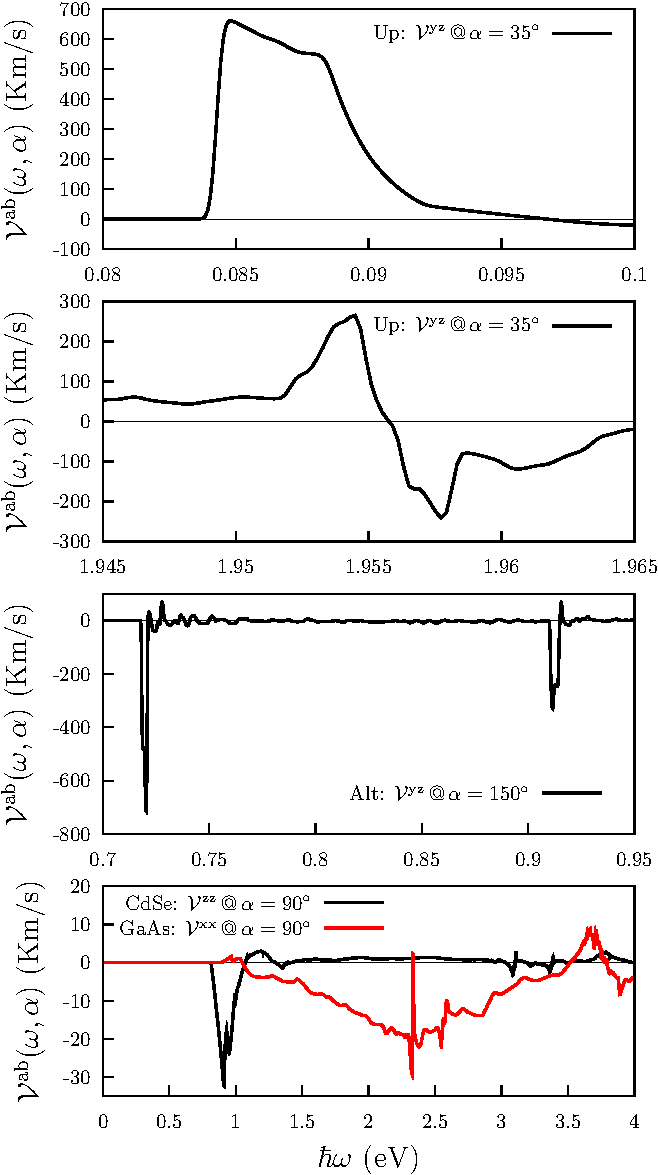
\includegraphics[width=\linewidth]{plots/vab-str-comp}
    
    \caption{Comparison of most intense responses of
    $\mathcal{V}^{\mathrm{ab}}$ for 2D \emph{alt} and \emph{up}, and bulk CdSe
    and GaAs structures and the corresponding polarization angles.}
    \label{fig:vab-str-comp}
\end{figure}

{\color{red}Using the Eq. \eqref{eq:vab-aw}, we calculated the
$\mathcal{V}^{\mathrm{ab}}(\omega,\alpha)$ response for the \emph{up} and
\emph{alt} 2D structures and for the CdSe and GaAs bulk systems; the results
are presented in Fig. \ref{fig:vab-str-comp}. The angle $\alpha$ presented in
the response of each structure is that for which the response is maximized in
each case.}
% 
From the figure we have that the onset of the response starts when the energy
of the incoming beam is the same of the gap energy.
% 
The most intense response corresponds to the \emph{up} structure centered at
0.088\,eV corresponding to the {\color{red} Mid Infrared (MIR)} radiation and
reaching a spin velocity of 87.2\,Km/s.
% 
In the other hand, for an energy range from 0.66\,eV to 3.0\,eV, corresponding
to energies of the {\color{red} Near Infrared (NIR) to visible radiation}, all
the four structures have contributions in the same order of magnitude.
% 
For this energy range the \emph{up} structure has two peaks centered at
1.94\,eV and 1.97\,eV reaching spin velocities of 22.2\,Km/s and -29.7\,Km/s,
respectively, and the \emph{alt} structure has two peaks centered at 0.72\,eV
and 0.91\,eV reaching spin velocities of -40.2\,Km/s and -32.9\,Km/s,
respectively.
% 
Then, for the bulk structures we have that the CdSe has only one intense
response centered at 0.91\,eV reaching a spin velocity of -26.9\,Km/s, and the
GaAs structure has a large and almost planar zone where the response is held
reaching the maximum for an incoming beam of energy of 2.31\,eV and resulting
in a spin velocity of -21.6\,Km/s.
% 
{\color{red} A negative quantity in the spin velocity means a change in the
spin polarization traveling in the opposite direction.
% 
In table \ref{tab:vab-str-comp} we present the comparison of this values for
the 2D and bulk structures. We found that the most intense response for the
spin velocity corresponds to the \emph{up} structure being 3.25 times more
intense than that of the CdSe and 4.03 times more intense than that of the GaAs
bulk structures. Also, the \emph{alt} structure has a response more intense
than the bulk systems but being less intense than the corresponding to the
\emph{up} one.}
% 


%%%%%%%%%%%%%%%%%%%%%%%%%%%%%%%%%%%%%%%%%%%%%%%%%%%%%%%%%%%%%%%%%%%%%%%%%%%%%%
%%%%%%%%%%%%%%%%%%%%%%%%%%%% Results: Fixing spin %%%%%%%%%%%%%%%%%%%%%%%%%%%%
%%%%%%%%%%%%%%%%%%%%%%%%%%%%%%%%%%%%%%%%%%%%%%%%%%%%%%%%%%%%%%%%%%%%%%%%%%%%%%


\subsection{Fixing spin} % (fold)
\label{sec:res-fixspin}


%%%%%%%%%%%%%%%%%%%%%%%%%%%%%%%%%%%%%%%%%%%%%%%%%%%%%%%%%%%%%%%%%%%%%%%%%%%%%%
%%%%%%%%%%%%%%%%%%%%%%%%%%% Res: fixing spin Up  %%%%%%%%%%%%%%%%%%%%%%%%%%%%%

\begin{figure}[t]
    \centering
    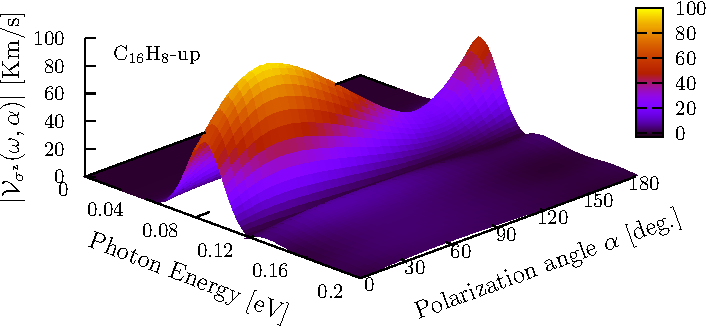
\includegraphics[width=\linewidth]{upplots/up-3d-svaz-1}
    \\
    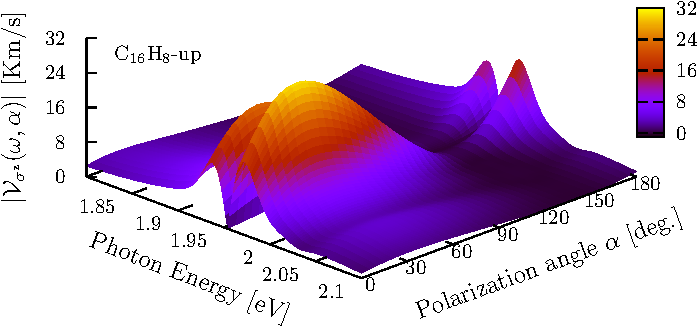
\includegraphics[width=\linewidth]{upplots/up-3d-svaz-2}

    \caption{$|\mathcal{V}_{\sigma^{\mathrm{z}}}(\omega,\alpha)|$ response
    as a function of the photon energy and polarization angle $\alpha$ for the
    \emph{up} structure for two energy ranges. The absolute maxima is located
    for an energy range from 0.08\,eV to 0.10\,eV, in the Far Infrared
    radiation range, and two local maxima from 1.90\,eV to 1.93\,eV and from
    1.96\,eV to 2.0\,eV, in the visible radiation range, all for polarization
    angles between $25^{\circ}$ and $50^{\circ}$.}
    \label{fig:up-3d-vsz}   
\end{figure}

\begin{figure}[t]
    \centering
    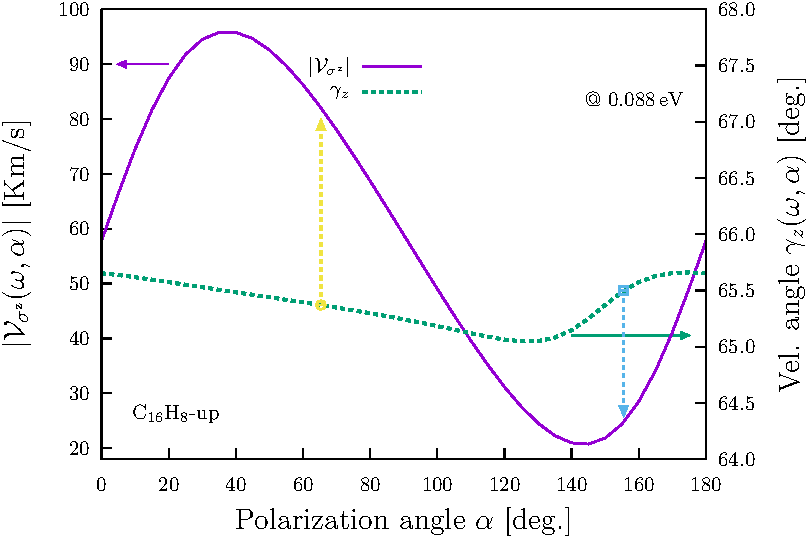
\includegraphics[width=\linewidth]{upplots/up-vaz-rag-1}
    \\
    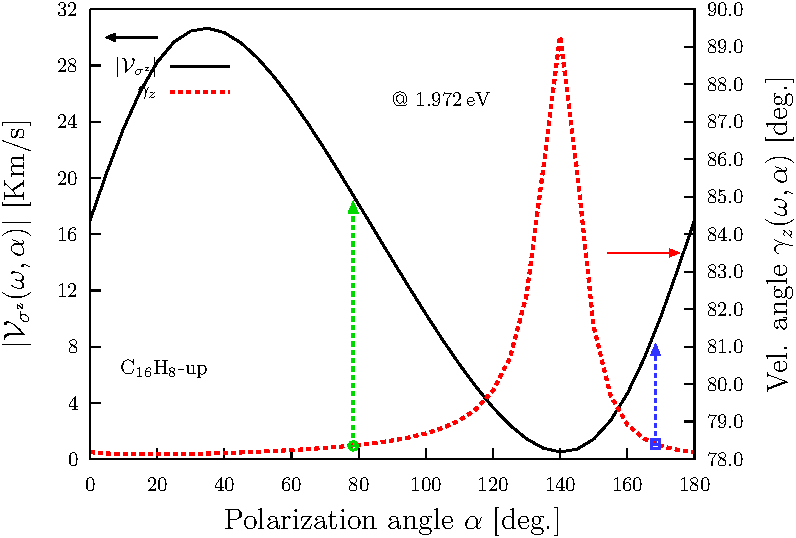
\includegraphics[width=\linewidth]{upplots/up-vaz-rag-2}

    \caption{Most intense response of
    $|\mathcal{V}_{\sigma^{\mathrm{z}}}(\omega,\alpha)|$ (top frames, right
    scale of figs (a) and (b)), the corresponding velocity angle
    $\gamma_{\mathrm{z}}(\omega,\alpha)$ (top frames, right scale), the
    collinear (circled box) and perpendicular (square box) angles, and the two
    components $\mathcal{V}^{\mathrm{xz}}(\omega,\alpha)$ and
    $\mathcal{V}^{\mathrm{yz}}(\omega,\alpha)$ (bottom frames) for the
    \emph{up} structure fixing the energy to 0.088\,eV. }
    \label{fig:up-vaz-rag}
\end{figure}

% %%%%%%%%%%%%%%%%%
% %% 0.0 eV - 0.16 eV  &  1.80 ev - 2.1 ev
% %% Description of UP |V_{s^z}| 3D
% %%%%%%%%%%%%%%%%%

{\color{red} Using the Eq. \eqref{eq:vs-mag}, we calculated the
$|\mathcal{V}_{\sigma^{\mathrm{b}}}(\omega,\alpha)|$ response and made the
analysis for the case when the spin is fixed in the $z$ coordinate, directed
perpendicularly to the surface of the \emph{up} and \emph{alt} structures.
Also, using the Eq. \eqref{eq:gamma-ang}, we determined the angle
$\gamma_{\mathrm{b}}(\omega,\alpha)$ where the spin-velocity is directed on the
surface of the each structure.}
% 

\textbf{Up structure}

We first analyzed two energy ranges in Fig. \ref{fig:up-3d-vsz} for the
\emph{up} structure, the first for an incoming energy beam from 0.0\,eV to
0.2\,eV (top panel)  which include the THz and the Mid Infrared (MIR)
radiation, where the absolute maximum of the
$|\mathcal{V}_{\sigma^{\mathrm{z}}}(\omega,\alpha)|$ response is obtained, and
the second for an energy range from 1.80\,eV to 2.1\,eV (bottom panel),
corresponding to visible radiation, where two local maxima are found.
% 
Making the analysis, we obtained that the zone where the maximum response is
held corresponds to a energy range of the incident beam from 0.084\,eV to
0.093\,eV and polarization angles $\alpha$ between $30^{\circ}$ and
$45^{\circ}$. Also the two local maxima are held for same beam polarization
angles but for an energy range between 1.90\,eV and 2.05\,eV. In the top frames
of top and bottom panels of Fig. \ref{fig:up-vaz-rag} we present in solid lines
the result of evaluate $|\mathcal{V}_{\sigma^{\mathrm{z}}}(\omega,\alpha)|$,
related to the left scale, fixing the energy of the incoming beam to 0.088\,eV
and 1.972\,eV, respectively, values for which the response is maximized for the
\emph{up} structure. In the same panels and frames we present in dashed lines,
related to the right scale, the corresponding velocity angle
$\gamma_{\mathrm{z}}(\omega,\alpha)$, and in the bottom frames of the panels we
present the corresponding components $\mathcal{V}^{\mathrm{xz}}(\omega,\alpha)$
and $\mathcal{V}^{\mathrm{yz}}(\omega,\alpha)$. Also we present two circled and
square boxes indicating the values where the angles of the spin velocity are
parallel (Eq. \ref{eq:gamma-par}) and perpendicular (Eq. \ref{eq:gamma-perp})
and the arrows are directed to the value of the response corresponding to those
angles.
% %%%%%%%%%%%%%%%%%
% %% 0.0 eV - 0.16 eV
% %% Description of UP |V_{s^z}| & gamma  vs. alpha agle
% %%%%%%%%%%%%%%%%%
From top panels of Figs. \ref{fig:up-3d-vsz} and \ref{fig:up-vaz-rag} we have
that the absolute maximum response for the \emph{up} structure is obtained for
an incoming beam with energy of 0.088\,eV and polarization angle
$\alpha=40^{\circ}$ resulting in a value of
$|\mathcal{V}_{\sigma^{\mathrm{z}}}(\omega,\alpha)|=95.8$\,Km/s coming from the
contribution of the components
$\mathcal{V}^{\mathrm{xz}}(\omega,\alpha)=39.8$\,Km/s and
$\mathcal{V}^{\mathrm{yz}}(\omega,\alpha)=87.2$\,Km/s for the spin polarized in
the $\mathrm{z}$ direction and having a velocity angle
$\gamma_{\mathrm{z}}(\omega,\alpha)=65^{\circ}$ on the first Cartesian quadrant
of the $xy$ plane.
% 
{\color{red} From the top panel of Fig. \ref{fig:up-vaz-rag} we have that the
velocity angle is almost constant for all the polarization angle range having
values of $\gamma_{\mathrm{z}}(\omega,\alpha) = 65.5^{\circ} \pm 0.5^{\circ}$.
In this panel the green circled box indicates the value for which the
polarization angle and the response direction angle are collinear corresponding
to $\gamma_{\mathrm{z}\parallel}(\omega,\alpha) = 65.5^{\circ}$ and resulting
in a value of the response of
$|\mathcal{V}_{\sigma^{\mathrm{z}}}(\omega,\alpha)| = 82.3$\,Km/s indicated by
the upward green arrow.
% 
Also the blue square box indicates the value for which the polarization angle
and the response angle are perpendicular being $\alpha=155.5^{\circ}$ and
$\gamma_{\mathrm{z}\perp}(\omega,\alpha)=65.5^{\circ}$; for this angle the
response has a value of $|\mathcal{V}_{\sigma^{\mathrm{z}}}(\omega,\alpha)| =
24.8$\,Km/s indicated by the blue downward arrow.}
% 
Now, from bottom panels of Figs. \ref{fig:up-3d-vsz} and \ref{fig:up-vaz-rag}
we have that the most intense local maximum of the response is obtained for an
incoming beam with energy of 1.972\,eV and same polarization angle
$\alpha=40^{\circ}$ resulting in a value of
$|\mathcal{V}_{\sigma^{\mathrm{z}}}(\omega,\alpha)|=30.3$\,Km/s. This comes
from a major contribution of the $\mathcal{V}^{\mathrm{yz}}(\omega,\alpha)$
component being directed in a velocity angle
$\gamma_{\mathrm{z}}(\omega,\alpha) = 78^{\circ}$ on the first Cartesian
Quadrant on the $xy$ plane.
% 
{\color{red} Again from the bottom panel of Fig. \ref{fig:up-vaz-rag} we found
that the velocity angle is almost constant at $78^{\circ}$ and has variations
of $1^{\circ}$ for polarization angles $0^{\circ} \leq \alpha \leq
100^{\circ}$. In this range the green circled box indicates the value for which
the polarization angle and the response direction angle are collinear
corresponding to $\gamma_{\mathrm{z}\parallel}(\omega,\alpha) = 78.5^{\circ}$
and having a response value of
$|\mathcal{V}_{\sigma^{\mathrm{z}}}(\omega,\alpha)| = 23.5$\,Km/s indicated
with the green upward arrow.
% 
Finally, the blue square box indicates the value for which the polarization
angle and the response angle are perpendicular being $\alpha=168.5^{\circ}$
$\gamma_{\mathrm{z}\perp}(\omega,\alpha) = 78.5^{\circ}$ and having a response
$|\mathcal{V}_{\sigma^{\mathrm{z}}}(\omega,\alpha)|=9.0$\,Km/s indicated with
the blue upward arrow.}
% 
We also made the analysis for the cases when the spin polarization is directed
along the $\mathrm{x}$ and $\mathrm{y}$ Cartesian coordinates but we do not
present here the corresponding plots. For those cases we have that the absolute
maxima responses are obtained for an energy of the incoming beam equal to
0.088\,eV and polarization angle $\alpha=40^{\circ}$ resulting in values of
$|\mathcal{V}_{\sigma^{\mathrm{x}}}(\omega,\alpha)|=37.4$\,Km/s and
$|\mathcal{V}_{\sigma^{\mathrm{y}}}(\omega,\alpha)|=24.8$\,Km/s.

%%%%%%%%%%%%%%%%%%%%%%%%%%%%%%%%%%%%%%%%%%%%%%%%%%%%%%%%%%%%%%%%%%%%%%%%%%%%%%
%%%%%%%%%%%%%%%%%%%%%%%%%%% Res: fixing spin Alt  %%%%%%%%%%%%%%%%%%%%%%%%%%%%

\begin{figure}[tb]
    \centering
    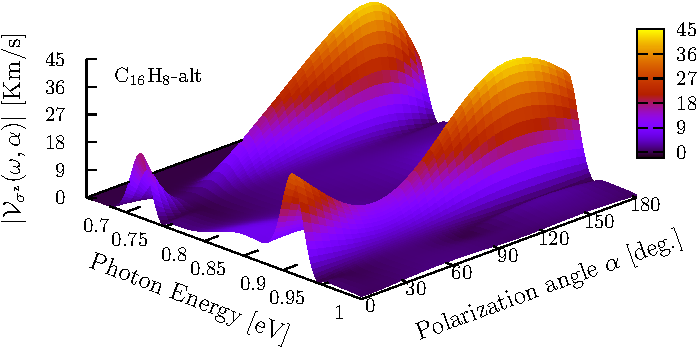
\includegraphics[width=\linewidth]{altplots/alt-3d-svaz}
    \caption{$|\mathcal{V}_{\sigma^{\mathrm{z}}}(\omega,\alpha)|$ response
    as a function of the photon energy and polarization angle $\alpha$  for the
    \emph{alt} structure. The local and the absolute maxima are located in the
    energy ranges from 0.67\,eV to 0.73\,eV and from 0.90\,eV to 0.93\,eV,
    respectively, and both in the Near Infrared and for polarization angles
    between $120^{\circ}$ and $150^{\circ}$.}
    \label{fig:alt-3d-vsb}
\end{figure}

\begin{figure}[t]
    \centering
    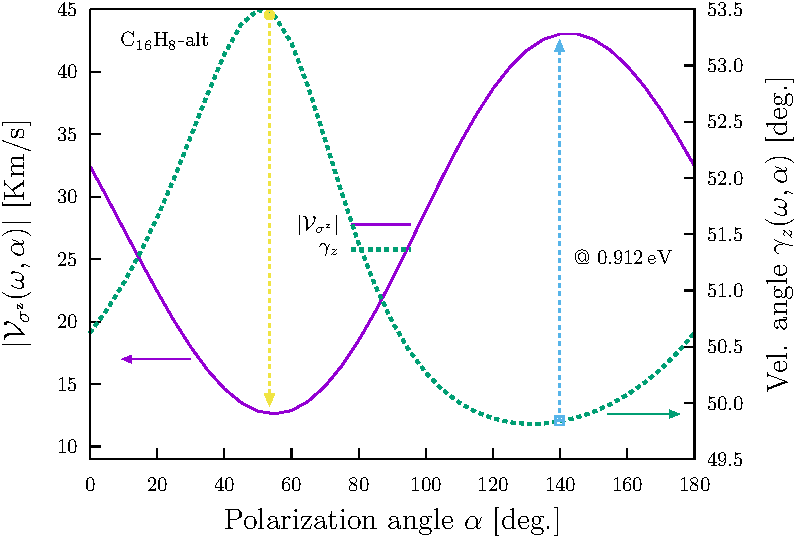
\includegraphics[width=\linewidth]{altplots/alt-vaz-rag}
    \caption{Most intense response of
    $|\mathcal{V}_{\sigma^{\mathrm{z}}}(\omega,\alpha)|$ (top frame, left
    scale) the corresponding velocity angle $\gamma_{\mathrm{z}}(\omega)$ (top
    frame, right scale), the collinear (circled box) and perpendicular (square
    box) angles, and the two components $\mathcal{V}^{\mathrm{xz}}(\omega)$ and
    $\mathcal{V}^{\mathrm{yz}}(\omega)$ (bottom frame) for the \emph{alt}
    structure fixing the energy to 0.912\,eV.}
    \label{fig:alt-vaz-rag}
\end{figure}

% %%%%%%%%%%%%%%%%%
% %% 0.0 eV - 0.16 eV  &  1.80 ev - 2.1 ev
% %% Description of ALT |V_{s^z}| 3D
% %%%%%%%%%%%%%%%%%

\textbf{Alt structure}

In Fig. \ref{fig:alt-3d-vsb} we analyzed the energy range for the incident beam
from 0.6\,eV to 1.0\,eV, corresponding to the NIR radiation, where the absolute
maximum of $|\mathcal{V}_{\sigma^{\mathrm{z}}}(\omega,\alpha)|$ response is
obtained for the \emph{alt} structure .
% From this figure we found that the zone where the absolute maximum response
% is held corresponds to a energy range from 0.90\,eV to 0.93\,eV and
% polarization angles $\alpha$ between $120^{\circ}$ and $150^{\circ}$. Also, a
% local maximum is obtained for the same polarization angles but for energies
% between 0.67\,eV and 0.75\,eV.
% %%%%%%%%%%%%%%%%%
% %% 0.0 eV - 0.16 eV
% %% Description of ALT |V_{s^z}| & gamma  vs. alpha agle
% %%%%%%%%%%%%%%%%%
% 
{\color{red} From Figs. \ref{fig:alt-3d-vsb} and \ref{fig:alt-vaz-rag} we have
that the absolute maximum response is obtained for an incoming beam with
polarization angle $\alpha=145^{\circ}$ reaching a velocity of
$|\mathcal{V}_{\sigma^{\mathrm{z}}}(\omega,\alpha)| = 43.0$\,Km/s for the spin
polarized in the $\mathrm{z}$ direction and resulting in a velocity angle
$\gamma_{\mathrm{z}}(\omega,\alpha)=50^{\circ}$ on the first Cartesian Quadrant
of the $xy$ plane.
% 
Also, from the top frame of Fig. \ref{fig:alt-vaz-rag} we found that the
velocity angle is centered at $51.5^{\circ}$ having variations of $\pm
2^{\circ}$ for the polarization angle range $0^{\circ} \leq
\alpha \leq 180^{\circ}$.
% 
As made in the previous analysis the circled box indicates the collinear angle
(Eq. \eqref{eq:gamma-par}) $\gamma_{\mathrm{z}\parallel}(\omega,\alpha) =
53.5^{\circ}$ corresponding a value of
$|\mathcal{V}_{\sigma^{\mathrm{z}}}(\omega,\alpha)| = 12.7$\,Km/s; the blue
square box indicates the perpendicular angles corresponding values
$\alpha=140^{\circ}$ and $\gamma_{\mathrm{z}\perp}(\omega,\alpha)=50^{\circ}$
with a value of $|\mathcal{V}_{\sigma^{\mathrm{z}}}
(\omega,\alpha)|=43.0$\,Km/s.}
% 
Again, for the cases in which the spin polarization is parallel to the surface
of the \emph{alt} structure was calculated but the plots are not presented
here. The absolute maxima for the cases when the spin polarization are directed
in the $\mathrm{x}$ and $\mathrm{y}$ direction are obtained for an energy of
the incoming beam equal to 0.912\,eV and polarization angle
$\alpha=145^{\circ}$ resulting in values of
$|\mathcal{V}_{\sigma^{\mathrm{x}}}(\omega,\alpha)|=27.1$\,Km/s and
$|\mathcal{V}_{\sigma^{\mathrm{y}}}(\omega,\alpha)|=33.2$\,Km/s.

%%%%%%%%%%%%%%%%%%%%%%%%%%%%%%%%%%%%%%%%%%%%%%%%%%%%%%%%%%%%%%%%%%%%%%%%%%%%%%
%%%%%%%%%%%%%%%%%%%%%%%%%% Results: Fixing velocity %%%%%%%%%%%%%%%%%%%%%%%%%%
%%%%%%%%%%%%%%%%%%%%%%%%%%%%%%%%%%%%%%%%%%%%%%%%%%%%%%%%%%%%%%%%%%%%%%%%%%%%%%


\subsection{Fixing velocity} % (fold)
\label{sec:res-fixvel}


%%%%%%%%%%%%%%%%%%%%%%%%%%%%%%%%%%%%%%%%%%%%%%%%%%%%%%%%%%%%%%%%%%%%%%%%%%%%%%
%%%%%%%%%%%%%%%%%%%%%%%%%%% Res: fixin vel Up  %%%%%%%%%%%%%%%%%%%%%%%%%%%%%%%

{\color{red} Now, using the Eq. \eqref{eq:vv-mag}, we calculated the
$|\mathcal{V}^{\mathrm{a}}(\omega,\alpha)|$ response and made the analysis for
the case when the velocity is fixed in the $x$ and $y$ direction over the
surface of the \emph{alt} and \emph{up} structures. Also, using the Eqns.
\eqref{eq:polar-ang} and \eqref{eq:azimuthal-ang}, we determined the polar
$\theta_{\mathrm{a}}(\omega,\alpha)$ and azimuthal
$\varphi_{\mathrm{a}}(\omega,\alpha)$ angles where the spin polarization is
directed.}


\textbf{Up structure.}
\begin{figure}[t]
    \centering
    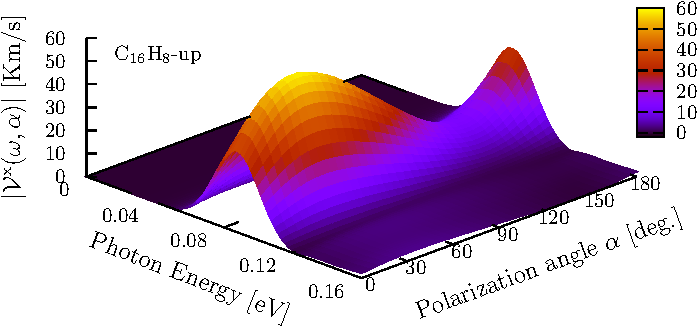
\includegraphics[width=\linewidth]{upplots/up-3d-vxb-1}
    \\
    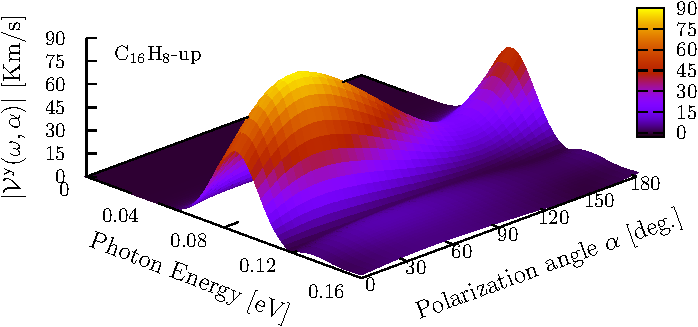
\includegraphics[width=\linewidth]{upplots/up-3d-vyb-1}
    
    \caption{ $|\mathcal{V}^{\mathrm{x}}(\omega,\alpha)|$ and
    $|\mathcal{V}^{\mathrm{y}}(\omega,\alpha)|$responses as a function of the
    photon energy and polarization angle $\alpha$ for the \emph{up} structure.
    The absolute maxima of both are localized in the energy range from 0.08\,eV
    to 0.10\,eV, in the Far  Infrared, and for polarization angles from
    $25^{\circ}$ to $50^{\circ}$.}
    \label{fig:up-3d-vva-1}
\end{figure}
\begin{figure}[t]
    \centering
    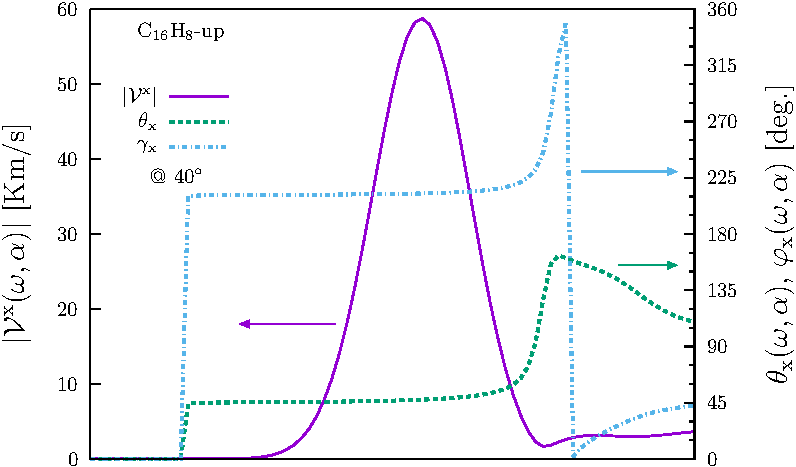
\includegraphics[width=\linewidth]{upplots/up-vxb-rtp-m1}
    \\
    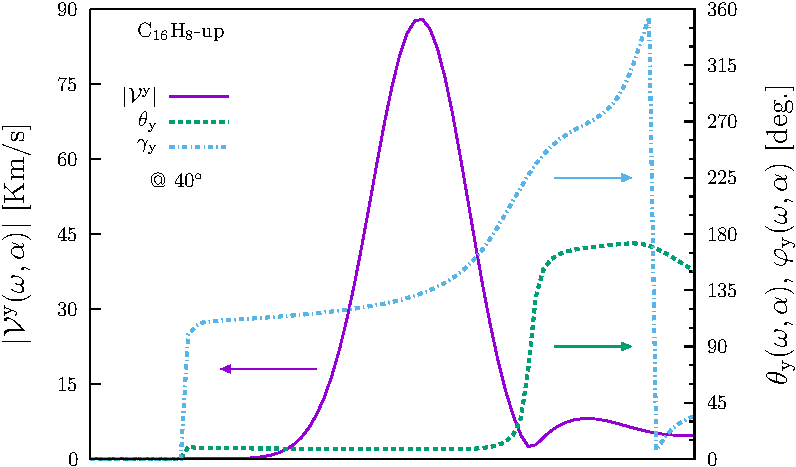
\includegraphics[width=\linewidth]{upplots/up-vyb-rtp-m1}
    
    \caption{Most intense response of
    $|\mathcal{V}^{\mathrm{x}}(\omega,\alpha)|$ and
    $|\mathcal{V}^{\mathrm{y}}(\omega,\alpha)|$ (top frames left scale of Figs.
    (a) and (b)), the corresponding polar $\varphi$ and azimuthal $\theta$
    angles (top frames right scale), and the corresponding three components
    (bottom frames) for the \emph{up} structure fixing the polarization angle
    to $\alpha=40^{\circ}$ to maximize the response.}
    \label{fig:up-vab-comp-rtp-1}
\end{figure}

% %%%%%%%%%%%%%%%%%
% %% 0.0 eV - 0.16 eV
% %% Description of UP |V^{a}| 3D
% %%%%%%%%%%%%%%%%%
In top and bottom panels of Fig. \ref{fig:up-3d-vva-1} we present the
$|\mathcal{V}^{\mathrm{x}}(\omega,\alpha)|$ and
$|\mathcal{V}^{\mathrm{y}}(\omega,\alpha)|$ spectra resulting from evaluate the
Eq. \eqref{eq:vv-mag} in the energy range for the incoming beam from 0.00\,eV
to 0.16\,eV for the \emph{up} structure.
%
From this figure we can see that for the zone between the energy range of
0.084\,eV-0.093\,eV and polarization angles between $30^{\circ}$ and
$45^{\circ}$ is the zone where the maximum response is held for both,
$|\mathcal{V}^{\mathrm{x}}(\omega,\alpha)|$ and
$|\mathcal{V}^{\mathrm{y}}(\omega,\alpha)|$.
% %%%%%%%%%%%%%%%%%
% %% 1.8 eV - 2.0 eV
% %% Description of UP |V^{a}|, components and RTP
% %%%%%%%%%%%%%%%%%

In the top frames of top and bottom panels of Fig. \ref{fig:up-vab-comp-rtp-1}
we present in solid lines the results of
$|\mathcal{V}^{\mathrm{x}}(\omega,\alpha)|$ and
$|\mathcal{V}^{\mathrm{y}}(\omega,\alpha)|$, related to the left scale, fixing
the polarization angle to $\alpha=40^{\circ}$ for which the response is
maximized. In the same panels and frames we present in dashed lines the
corresponding polar $\theta_{a}(\omega,\alpha)$ and azimuthal
$\varphi_{a}(\omega,\alpha)$ spin polarization angles related to the right
scale. Also, in the bottom frames of the panels we present the corresponding
components $\mathcal{V}^{\mathrm{xx}}(\omega,\alpha)$,
$\mathcal{V}^{\mathrm{xy}}(\omega,\alpha)$,
$\mathcal{V}^{\mathrm{xz}}(\omega,\alpha)$, and
$\mathcal{V}^{\mathrm{yx}}(\omega,\alpha)$,
$\mathcal{V}^{\mathrm{yy}}(\omega,\alpha)$,
$\mathcal{V}^{\mathrm{yz}}(\omega,\alpha)$.
\begin{figure}[t]
    \centering
    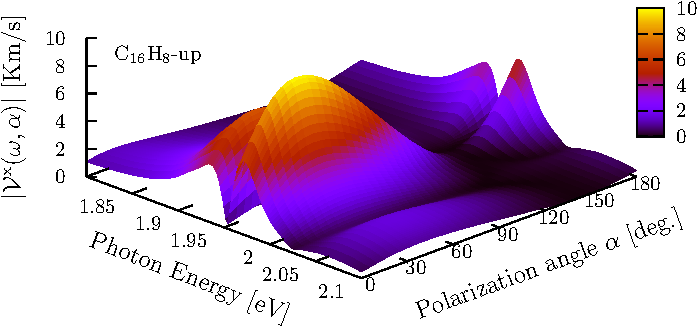
\includegraphics[width=\linewidth]{upplots/up-3d-vxb-2}
    \\
    
\includegraphics[width=\linewidth]{upplots/up-3d-vyb-2}
    
    \caption{$|\mathcal{V}^{\mathrm{x}}(\omega,\alpha)|$ (top panel) and
    $|\mathcal{V}^{\mathrm{y}}(\omega,\alpha)|$ (bottom panel)  as a function
    of the photon energy and polarization angle $\alpha$ for the \emph{up}
    structure. Two local maxima of both responses are localized in the energy
    range from 1.90\,eV to 1.93\,eV and from 1.96\,eV to 2.0\,eV, in the
    visible radiation range, and for polarization angles between $25^{\circ}$
    and $50^{\circ}$.}
    \label{fig:up-3d-vva-2}
\end{figure}
\begin{figure}[t]
    \centering
    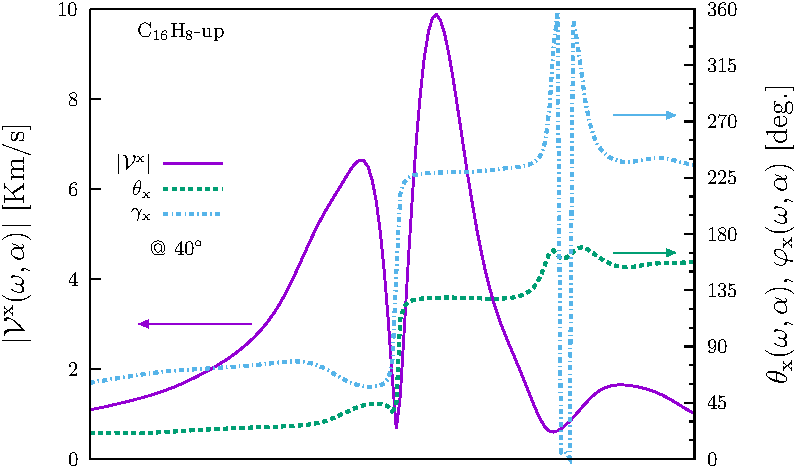
\includegraphics[width=\linewidth]{upplots/up-vxb-rtp-m2}
    \\
    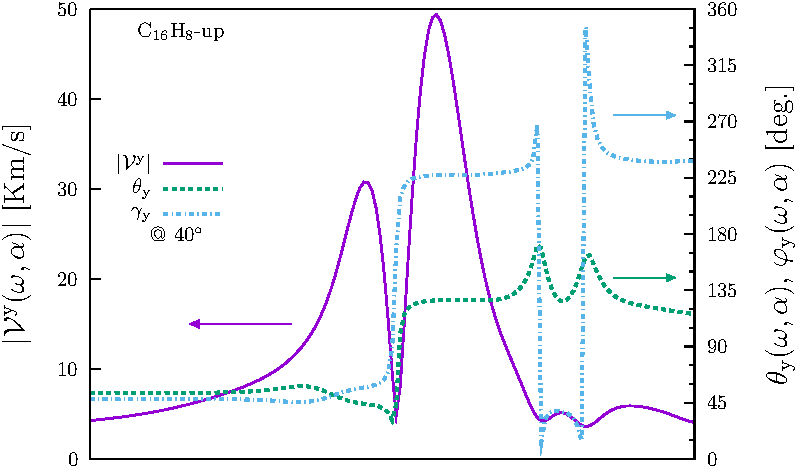
\includegraphics[width=\linewidth]{upplots/up-vyb-rtp-m2}
    
    \caption{Intense response of
    $|\mathcal{V}^{\mathrm{x}}(\omega,\alpha)|$ and
    $|\mathcal{V}^{\mathrm{y}}(\omega,\alpha)|$ (top frames left scale of Figs.
    (a) and (b)), the corresponding polar $\varphi$ and azimuthal $\theta$
    angles (top frames right scale), and the corresponding three components
    (bottom frames) for the \emph{up} structure fixing the polarization angle
    to $\alpha=40^{\circ}$ to maximize the response.}

    \label{fig:up-vab-comp-rtp-2}
\end{figure}
% %%%%%%%%%%%%%%%%%
% %% 1.8 eV - 2.0 eV
% %% Description of UP |V^{a}|, components and RTP
% %%%%%%%%%%%%%%%%%
From the top panel of Fig. \ref{fig:up-vab-comp-rtp-1} we have that for an
incoming bean with energy of 0.088\,eV the three components have similar
contributions with values of
% 
$\mathcal{V}^{\mathrm{xx}}(\omega,\alpha)=-36.5$\,Km/s,
$\mathcal{V}^{\mathrm{xy}}(\omega,\alpha)=-23.2$\,Km/s, and
$\mathcal{V}^{\mathrm{xz}}(\omega,\alpha)= 39.8$\,Km/s resulting in a response
$|\mathcal{V}^{\mathrm{x}}(\omega,\alpha)|=58.7$\,Km/s being this value the
absolute maximum obtained when the spin-velocity is fixed in the $x$ direction.
% 
{\color{red} To this value corresponds polar and azimuthal spin polarization
angles of $\theta_{\mathrm{x}}(\omega,\alpha)=47$ and
$\varphi_{\mathrm{x}}(\omega,\alpha)=212$, respectively, being directed upward
the third Cartesian quadrant of the $xy$ plane.
% 
Also from this figure we have that those angles values are held for almost all
the peak of the response having variations of $\pm 2^{\circ}$ each one.
% 
Now, from the bottom panel of Fig. \ref{fig:up-vab-comp-rtp-1} we have that the
components have contributions of
% 
$\mathcal{V}^{\mathrm{yx}}(\omega,\alpha)= -7.9$\,Km/s 
$\mathcal{V}^{\mathrm{yy}}(\omega,\alpha)=  8.6$\,Km/s, and
$\mathcal{V}^{\mathrm{yz}}(\omega,\alpha)= 87.2$\,Km/s 
% 
resulting in a response $|\mathcal{V}^{\mathrm{y}}(\omega,\alpha)|=87.9$\,Km/s.
This value is the absolute maximum obtained when the spin-velocity is fixed in
the $\mathrm{y}$ direction and is 1.5 times more intense than the maximum of
$|\mathcal{V}^{\mathrm{x}}(\omega,\alpha)|$ for this structure. To this
absolute maximum corresponds spin polarization polar and azimuthal angles
$\theta_{\mathrm{y}}(\omega,\alpha) = 8^{\circ}$ and
$\varphi_{\mathrm{y}}(\omega,\alpha) = 133^{\circ}$ being directed the spin
almost perpendicularly over the $xy$ plane and  localized on the first
Cartesian quadrant.}
% 
In a different way than in the $|\mathcal{V}^{\mathrm{x}}(\omega,\alpha)|$ case
for the $|\mathcal{V}^{\mathrm{y}}(\omega,\alpha)|$ only the polar angle is
held at $8^{\circ}$ for the peak of the response having variations of $\pm
2^{\circ}$ but the azimuthal angle changes from $99^{\circ}$ to $176^{\circ}$
having a value of $133^{\circ}$ for the maximum.
% 
We also found that since the onset of the response till an energy for the
incoming beam of 0.118\,eV the components of both responses, have no change in
the spin polarization-velocity direction. Finally, after this last energy value
the responses go to zero.
% %%%%%%%%%%%%%%%%%
% %% 1.80 eV - 2.10 eV
% %% Description of UP |V^{a}| 3D
% %%%%%%%%%%%%%%%%%
Also there is another energy range of interest for an incoming energy beam from
1.80\,eV to 2.10\,eV, corresponding to visible radiation, presented in Fig.
\ref{fig:up-3d-vva-2} where two local of both responses are obtained for the
\emph{up} structure for energies of 1.934\,eV and 1.972\,eV
fixing again the polarization angle to $40^{\circ}$.
% %%%%%%%%%%%%%%%%
% %% Starting description of UP |V^{x}|, components and RTP
% %%%%%%%%%%%%%%%%
{\color{red} We found that for both cases the components have similar
contributions for each response and for 1.934\,eV result in values of
$|\mathcal{V}^{\mathrm{x}}(\omega,\alpha)| = 6.6$\,Km/s for the spin velocity
moving along the $x$ direction with polar and azimuthal spin polarization
angles $\theta_{\mathrm{x}}(\omega,\alpha)= 42^{\circ}$ and
$\varphi_{\mathrm{x}}(\omega,\alpha)=59^{\circ}$ being the spin directed over
the first Cartesian quadrant of the $xy$ plane;
% 
for the spin moving along the $\mathrm{y}$ direction we have a response
$|\mathcal{V}^{\mathrm{y}}(\omega,\alpha)|=28.7$\,Km/s with polar and azimuthal
spin polarization angles $\theta_{\mathrm{y}}(\omega,\alpha)=45^{\circ}$ and
$\varphi_{\mathrm{y}}(\omega,\alpha)=56^{\circ}$ being  the spin directed over
the first Cartesian quadrant of the $xy$ plane.
% 
Alike, for an incoming energy beam of 1.972\,eV we found the second and more
intense local maxima for which all the components have similar contributions
for both responses.
% 
This result in values of $|\mathcal{V}^{\mathrm{x}}(\omega,\alpha)| =
9.9$\,Km/s and $|\mathcal{V}^{\mathrm{y}}(\omega,\alpha)| = 49.4$\,Km/s with
spin polarization angles $\theta_{\mathrm{x}}(\omega,\alpha) = 129^{\circ}$,
$\varphi_{\mathrm{x}}(\omega,\alpha)=229^{\circ}$,
$\theta_{\mathrm{y}}(\omega,\alpha) = 127^{\circ}$ and
$\varphi_{\mathrm{y}}(\omega,\alpha)=227^{\circ}$ being the spin directed
downward the third Cartesian quadrant of the $xy$ plane when it moves in the
$x$ direction and downward the third Cartesian quadrant when it moves along the
$y$ direction.}
% 
Also all the components of the responses keep the spin polarization positive
till an energy of the incoming beam equal to 1.954\,eV when the spin
polarization and current changes the direction. After an energy of 2.05\,eV
both responses goes to zero.

%%%%%%%%%%%%%%%%%%%%%%%%%%%%%%%%%%%%%%%%%%%%%%%%%%%%%%%%%%%%%%%%%%%%%%%%%%%%%%
%%%%%%%%%%%%%%%%%%%%%%%%%%% Res: fixin vel Alt  %%%%%%%%%%%%%%%%%%%%%%%%%%%%%%%

\textbf{Alt structure.}
\begin{figure}[tb]
    \centering
    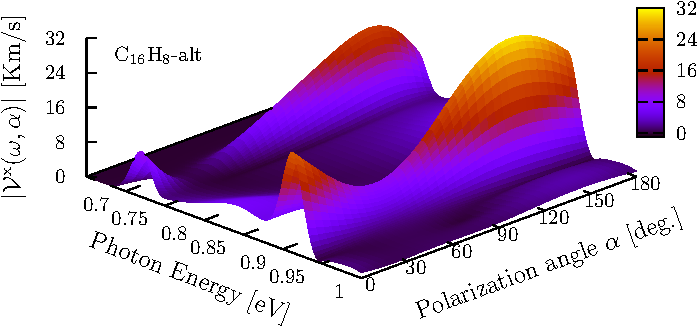
\includegraphics[width=\linewidth]{altplots/alt-3d-vxb}
    \\
    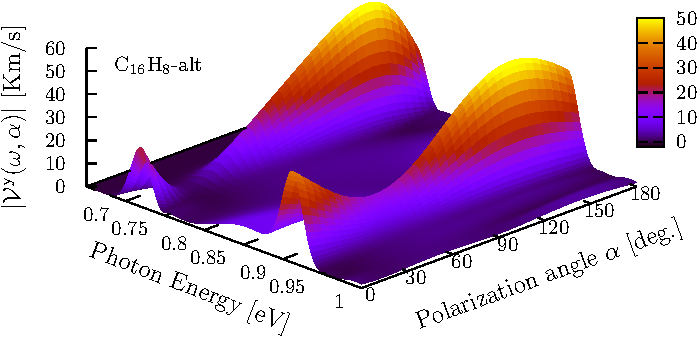
\includegraphics[width=\linewidth]{altplots/alt-3d-vyb}
    
    \caption{$|\mathcal{V}^{\mathrm{x}}(\omega,\alpha)|$ (top panel) and
    $|\mathcal{V}^{\mathrm{y}}(\omega,\alpha)|$ (bottom panel)  as a function
    of the photon energy and polarization angle $\alpha$ for the \emph{alt}
    structure. The local and the absolute maxima are located in the energy
    ranges from 0.67\,eV to 0.73\,eV and from 0.90\,eV to 0.93\,eV,
    respectively, and both in the Near Infrared and for polarization angles
    between $120^{\circ}$ and $150^{\circ}$.}
    \label{fig:alt-3d-vva}
\end{figure}

\begin{figure}[tb]
    \centering
    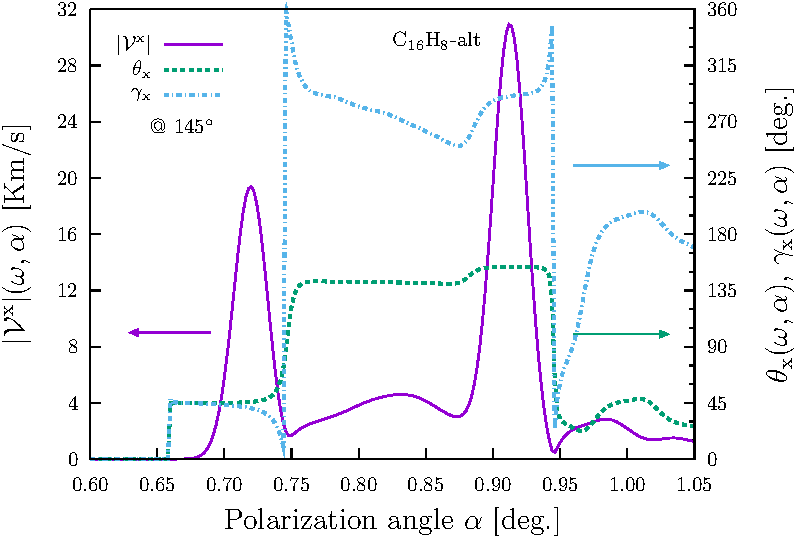
\includegraphics[width=\linewidth]{altplots/alt-vxb-rtp-m}
    \\
    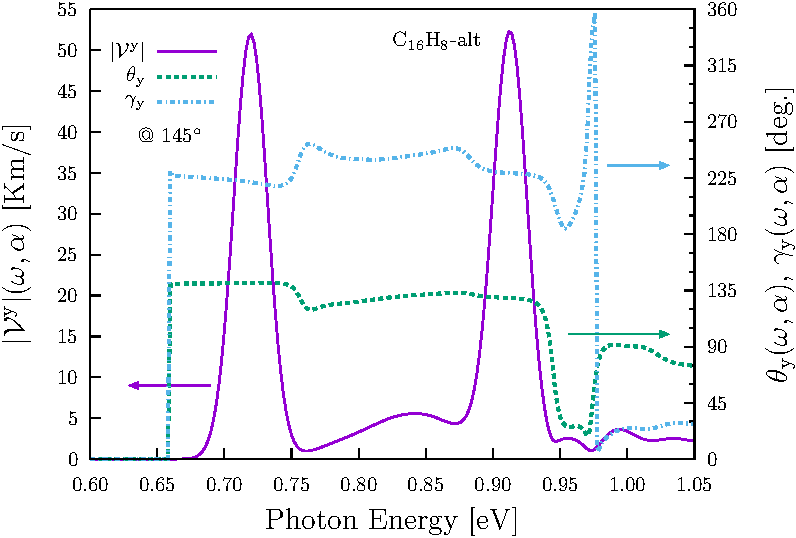
\includegraphics[width=\linewidth]{altplots/alt-vyb-rtp-m}

    \caption{Most intense response of
    $|\mathcal{V}^{\mathrm{x}}(\omega,\alpha)|$ and
    $|\mathcal{V}^{\mathrm{y}}(\omega,\alpha)|$ (top frames left scale of Figs.
    (a) and (b)), the corresponding polar $\varphi$ and azimuthal $\theta$
    angles (top frames right scale), and the corresponding three components
    (bottom frames) for the \emph{alt} structure fixing the polarization angle
    to $\alpha=145^{\circ}$ to maximize the response.}
    \label{fig:alt-vab-comp-rtp}
\end{figure}

% %%%%%%%%%%%%%%%%%
% %% Description of ALT |V^{a}| 3D
% %%%%%%%%%%%%%%%%%
{\color{red} For the \emph{alt} structure we analyzed the energy range from
0.6\,eV to 1.0\,eV in Fig. \ref{fig:alt-3d-vva}, corresponding to the NIR
radiation, where we found a local maxima and the most intense responses for
$|\mathcal{V}^{\mathrm{x}}(\omega,\alpha)|$ and
$|\mathcal{V}^{\mathrm{a}}(\omega,\alpha)|$.}
%
From this figure we can see that for the zone between the energy range of
0.90\,eV-0.93\,eV and polarization angles between 120$^{\circ}$ and
150$^{\circ}$ is the zone where the maximum for both responses is held.
% %%%%%%%%%%%%%%%%
% %% Starting description of ALT |V^{a}|, components and RTP
% %%%%%%%%%%%%%%%%
In the top frames of top and bottom panels of Fig. \ref{fig:alt-vab-comp-rtp}
we present the spectra of $|\mathcal{V}^{\mathrm{x}}(\omega,\alpha)|$ and
$|\mathcal{V}^{\mathrm{y}}(\omega,\alpha)|$ fixing the polarization angle to
$\alpha=145^{\circ}$ for which the response is maximized and its corresponding
polar and azimuthal angles; in the bottom frames of same panels we present the
corresponding three components $\mathcal{V}^{\mathrm{xx}}(\omega,\alpha)$,
$\mathcal{V}^{\mathrm{xy}}(\omega,\alpha)$,
$\mathcal{V}^{\mathrm{xz}}(\omega,\alpha)$,
$\mathcal{V}^{\mathrm{yx}}(\omega,\alpha)$,
$\mathcal{V}^{\mathrm{yy}}(\omega,\alpha)$ and
$\mathcal{V}^{\mathrm{yz}}(\omega,\alpha)$.
% 
{\color{red} Making the analysis when the energy of the incoming beam is
0.720\,eV we have similar contributions from the components when the sping
velocity is along the $x$ diection and a major contribution from
$\mathcal{V}^{\mathrm{yz}}(\omega,\alpha)$ when the spin velocity is dierected
alog $y$ Cartesian axis. This result in values of
$|\mathcal{V}^{\mathrm{x}}(\omega,\alpha)| = 19.4$\,Km/s and
$|\mathcal{V}^{\mathrm{y}}(\omega,\alpha)| = 51.9$\,Km/s with spin polarization
angles $\theta_{\mathrm{x}}(\omega,\alpha) = 46^{\circ}$,
$\varphi_{\mathrm{x}}(\omega,\alpha) = 41^{\circ}$,
$\theta_{\mathrm{y}}(\omega,\alpha) = 141^{\circ}$ and
$\varphi_{\mathrm{y}}(\omega,\alpha) = 222^{\circ}$ being the spin polarization
directed over the first Cartesian quadrant of the $xy$ plane when the spin
velocity is directed along $x$ and directed downward the third Cartesian
quadrant when the spin velocity is directed along $y$.
% 
Then, for an energy of 0.912\,eV we have values of
$|\mathcal{V}^{\mathrm{x}}(\omega,\alpha)|=30.9$\,Km/s and
$|\mathcal{V}^{\mathrm{y}}(\omega,\alpha)| = 52.3$\,Km/s. The first of them
have a major contribution from the $\mathcal{V}^{\mathrm{xz}}(\omega,\alpha)$
component and the second one having similar contributions from all of three
components. They result in polar and azimuthal angles
$\theta_{\mathrm{x}}(\omega,\alpha) = 154^{\circ}$,
$\varphi_{\mathrm{x}}(\omega,\alpha) = 290^{\circ}$,
$\theta_{\mathrm{y}}(\omega,\alpha) = 129^{\circ}$ and
$\varphi_{\mathrm{y}}(\omega,\alpha) = 229^{\circ}$ being the spin polarization
directed downward the fourth Cartesian quadrant of the $xy$ plane when the spin
velocity is directed along $x$ and downward the third Cartesian quadrant of the
$xy$ plane when the spin velocity is directed along $y$.}
% 
Finally we have that the three components of $|\mathcal{V}^{\mathrm{y}}|$ are
negative keeping the same spin polarization and velocity direction since the
onset of the response to a energy of the incoming beam of 0.886\,eV when the
response decreases and goes to zero.

%%%%%%%%%%%%%%%%%%%%%%%%%%%%%%%%%%%%%%%%%%%%%%%%%%%%%%%%%%%%%%%%%%%%%%%%%%%%%%
%%%%%%%%%%%%%%%%%%%%%%%%%% Res: Layer-by-layer  %%%%%%%%%%%%%%%%%%%%%%%%%%%%%%
%%%%%%%%%%%%%%%%%%%%%%%%%%%%%%%%%%%%%%%%%%%%%%%%%%%%%%%%%%%%%%%%%%%%%%%%%%%%%%

\section{Layer-by-layer analysis} % (fold)
\label{sec:res-layer_by_layer_analysis}

{\color{blue} As mentioned before in in the beginning of this section the
\emph{up} and \emph{alt} structures presented here was divided into layers to
analyze the layer-by-layer contribution for
$|\mathcal{V}_{\sigma^{\mathrm{z}}}(\omega,\alpha)|$ and
$|\mathcal{V}^{\mathrm{a}}(\omega,\alpha)|$. Here we present the decomposition
only for $|\mathcal{V}_{\sigma^{\mathrm{z}}}(\omega,\alpha)|$ and for the
corresponding components of the \emph{up} structure in Figs. 
% 
\ref{fig:up-vsz-lay-1} and \ref{fig:up-vsz-lay-2} and for the \emph{alt}
structure in Fig. \ref{fig:alt-vsz-lay}. The
$|\mathcal{V}_{\sigma^{\mathrm{z}}}(\omega,\alpha)|$ response presented in
those figures is the same than the presented in top frames of Figs.
% 
\ref{fig:up-vaz-rag} and \ref{fig:alt-vaz-rag} but now compared with the
layered responses.
% 
}
% 
\begin{figure}[t]
    \centering
    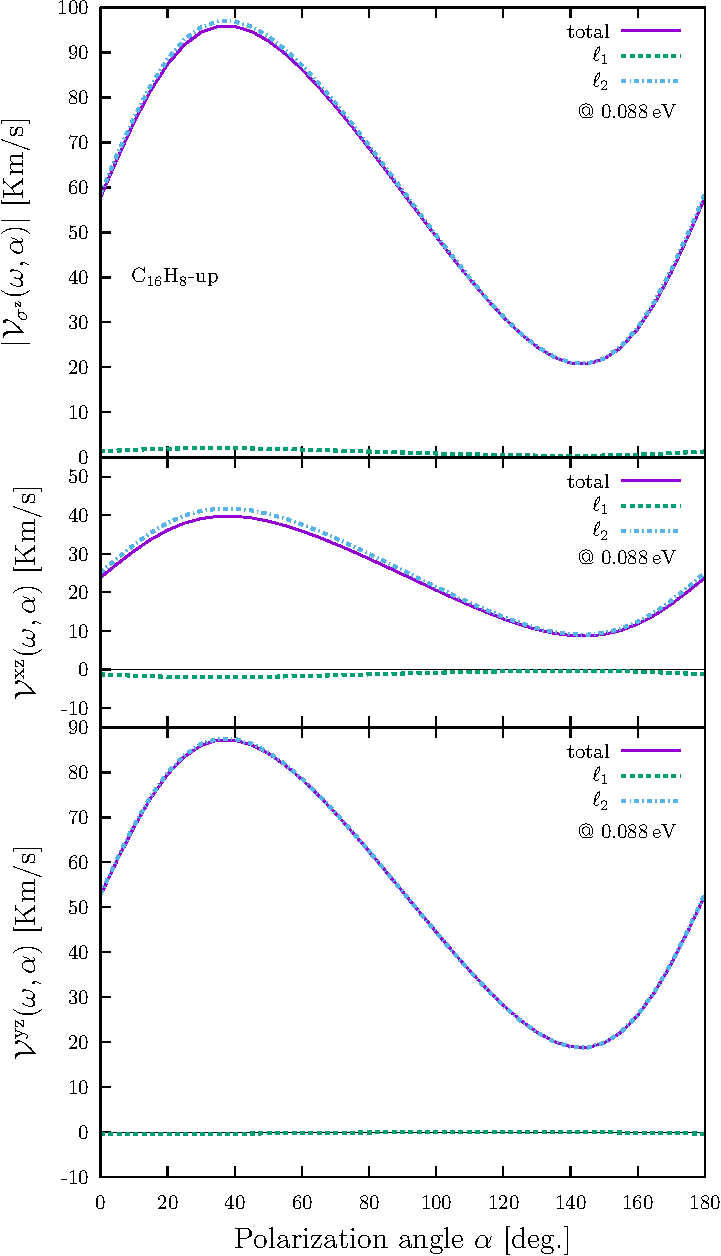
\includegraphics[width=\linewidth]{upplots/up-svaz-lay-1}
    
    \caption{Layer-by-layer contribution of the
    $|\mathcal{V}_{\sigma^{\mathrm{z}}}(\omega,\alpha)|$ response (top frame)
    for the \emph{up} structure as a function of the polarization angle
    $\alpha$ for the energy fixed to 0.088\,eV for which the absolute maximum
    is obtained.
    % 
    The corresponding layered contributions for the
    $\mathcal{V}^{\mathrm{xz}}(\omega,\alpha)$ and
    $\mathcal{V}^{\mathrm{zy}}(\omega,\alpha)$ components are presented in the
    central and bottom frames.}
    \label{fig:up-vsz-lay-1}
\end{figure}

\begin{figure}[t]
    \centering
    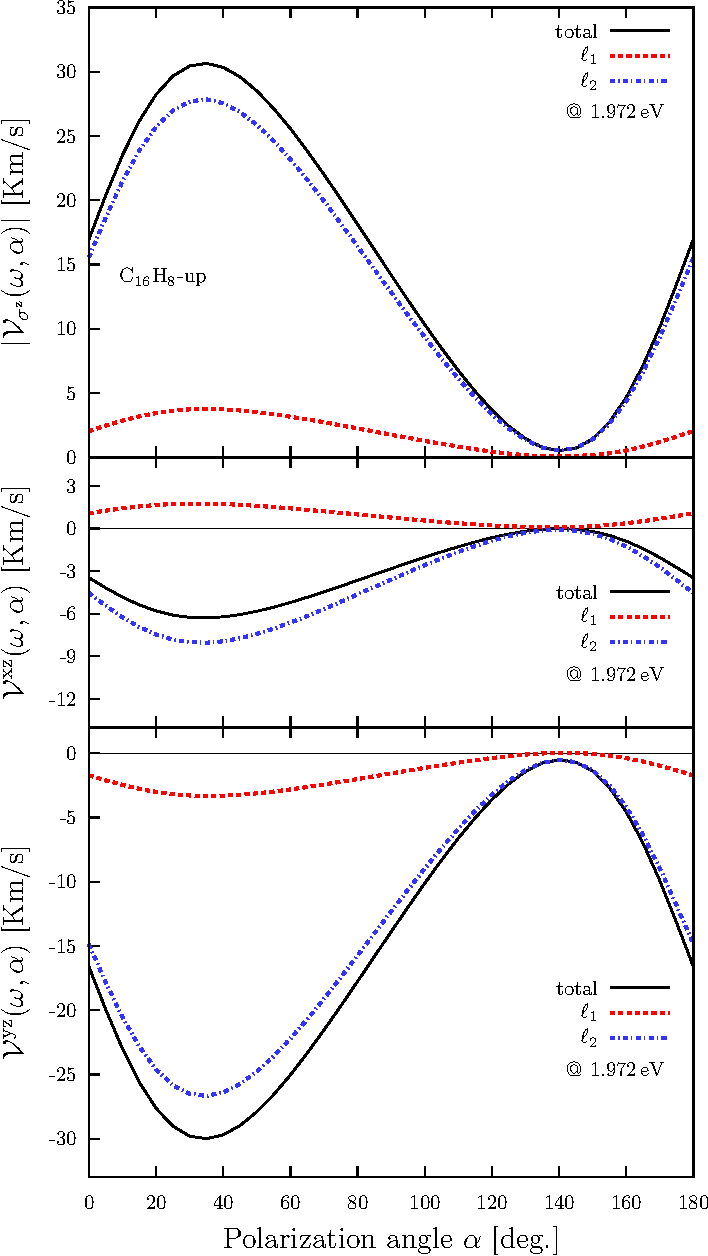
\includegraphics[width=\linewidth]{upplots/up-svaz-lay-2}
    
    \caption{Layer-by-layer contribution of the
    $|\mathcal{V}_{\sigma^{\mathrm{z}}}(\omega,\alpha)|$ response (top frame)
    for the \emph{up} structure as a function of the polarization angle
    $\alpha$ for the energy fixed to 1.972\,eV for which a local maximum is
    obtained.
    % 
    The corresponding layered contributions for the
    $\mathcal{V}^{\mathrm{xz}}(\omega,\alpha)$ and
    $\mathcal{V}^{\mathrm{zy}}(\omega,\alpha)$ components are presented in the
    central and bottom frames.}
    \label{fig:up-vsz-lay-2}
\end{figure}

\begin{figure}[t]
    \centering
    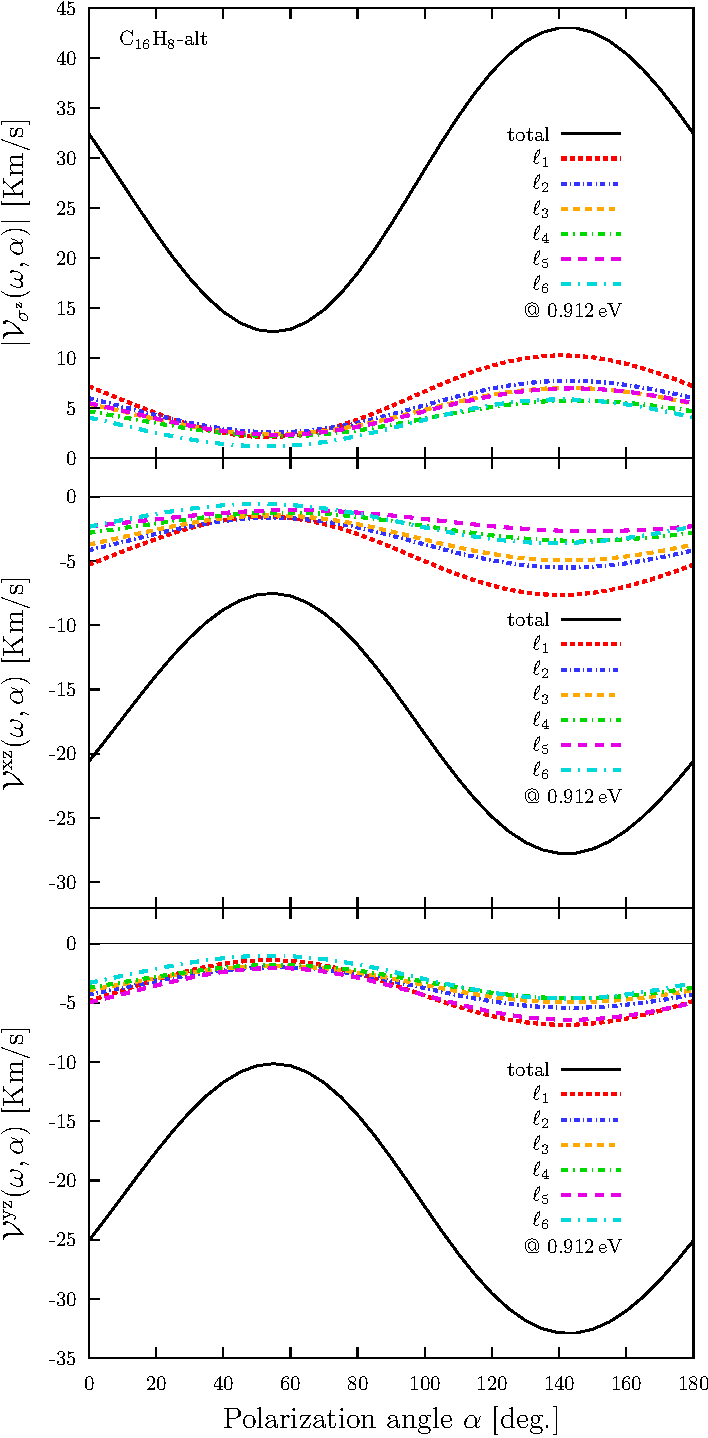
\includegraphics[width=\linewidth]{altplots/alt-svaz-lay}
    
\caption{Layer-by-layer contribution of the
    $|\mathcal{V}_{\sigma^{\mathrm{z}}}(\omega,\alpha)|$ response (top frame)
    for the \emph{alt} structure as a function of the polarization angle
    $\alpha$ for the energy fixed to 0.912\,eV for which the absolute maximum
    is obtained.
    % 
    The corresponding layered contributions for the
    $\mathcal{V}^{\mathrm{xz}}(\omega,\alpha)$ and
    $\mathcal{V}^{\mathrm{zy}}(\omega,\alpha)$ components are presented in the
    central and bottom frames.}
    \label{fig:alt-vsz-lay}
\end{figure}
% 

% %%%%%%%%%%%%%%%%
% %% Description of Up layer |V_{s^z}|
% %%%%%%%%%%%%%%%%
{\color{blue} From the central and bottom frames of Fig. \ref{fig:up-vsz-lay-1}
we have that when the energy is fixed to 0.088\,eV almost all the response of
the $\mathcal{V}^{\mathrm{xz}}(\omega,\alpha)$ component comes from the second
layer comprised by carbon atoms having a minimal reduction produced by the
hydrogen layer. Also, the $\mathcal{V}^{\mathrm{yz}}(\omega,\alpha)$ response,
presented in bottom frame of same figure, is produced only by the carbon layer.
This result in a total response
$|\mathcal{V}_{\sigma^{\mathrm{z}}}(\omega,\alpha)| = 95.8$\,Km/s coming from
the carbon layer and being minimally reduced by the hydrogen layer as shown in
the top frame of this figure.
% 
Now, for the same structure but now fixing the energy to 1.972\,eV we have from
the central frame of Fig. \ref{fig:up-vsz-lay-2} that the the carbon layer
produces the response of the $\mathcal{V}^{\mathrm{zx}}(\omega,\alpha)$
component being decreased by the hydrogen layer. Opposite to that, in the
bottom frame of same figure we obtained that the response of the carbon and
hydrogen layer are not inverse and then contributing both to the total response
of $\mathcal{V}^{\mathrm{yz}}(\omega,\alpha)$. Then, in the top frame of this
figure we have that the major contribution to the
$|\mathcal{V}_{\sigma^{\mathrm{z}}}(\omega,\alpha)|$ comes from the carbon
layer with but being in this case reinforced by the contribution of the
hydrogen layer and resulting in a value of 30.3\,Km/s}
% %%%%%%%%%%%%%%%%
% %% Description of ALT layer |V^{yz}|
% %%%%%%%%%%%%%%%%
{\color{blue}
Finally, for the \emph{alt} structure we have that the six layers contribute
with similar magnitudes and reinforce the
$\mathcal{V}^{\mathrm{xz}}(\omega,\alpha)$ and
$\mathcal{V}^{\mathrm{yz}}(\omega,\alpha)$ components resulting in a total
response $\mathcal{V}^{\mathrm{xz}}(\omega,\alpha) = 43$\,Km/s.
}


%%%%%%%%%%%%%%%%%%%%%%%%%%%%%%%%%%%%%%%%%%%%%%%%%%%%%%%%%%%%%%%%%%%%%%%%%%%%%%
%%%%%%%%%%%%%%%%%%%%%%%%%%%%%%%%%%%%%%%%%%%%%%%%%%%%%%%%%%%%%%%%%%%%%%%%%%%%%%
%%%%%%%%%%%%%%%%%%%%%%%%%%                          %%%%%%%%%%%%%%%%%%%%%%%%%%
%%%%%%%%%%%%%%%%%%%%%%%%%%   C O N C L U S I O N S  %%%%%%%%%%%%%%%%%%%%%%%%%%
%%%%%%%%%%%%%%%%%%%%%%%%%%                          %%%%%%%%%%%%%%%%%%%%%%%%%%
%%%%%%%%%%%%%%%%%%%%%%%%%%%%%%%%%%%%%%%%%%%%%%%%%%%%%%%%%%%%%%%%%%%%%%%%%%%%%%
%%%%%%%%%%%%%%%%%%%%%%%%%%%%%%%%%%%%%%%%%%%%%%%%%%%%%%%%%%%%%%%%%%%%%%%%%%%%%%


%%%%%%%%%%%%%%%%%%%%%%%%%%%%%%%%%%%%%%%%%%%%%%%%%%%%%%%%%%%%%%%%%%%%%%%%%%%%%%
%%%%%%%%%%%%%%%%%%%%%%%%%%%%%%%%%%%%%%%%%%%%%%%%%%%%%%%%%%%%%%%%%%%%%%%%%%%%%%

\section{Conclusions} % (fold)
\label{sec:conclusions}

Spintronics devices are based on the control of spin and electrical charge
through electrical and optical methods.
% 
Semiconductor spintronics gives the development possibility of devices that can
perform high-volume information manipulation, processing, and storage, for
computing and communications technologies. \cite{awschalomNP2007}
% 
We have performed an \emph{ab initio} calculation for the SVI by one-photon
absorption of linearly polarized light in the \emph{up} and \emph{alt} 2D
hydrogenated graphene structures that could result in spintronics devices
development. This effect does not seem to have been reported previously.
% 
We calculated the responses for two cases: when the spin polarization is fixed
along the Cartesian coordinates and when the spin velocity is directed along
the $x$ and $y$ Cartesian directions on the $xy$ surface of the structures. We
found that  the SVI is very susceptible to the characteristics of the
structures presenting an anisotropic behavior.
% 
We found that for both structures it is possible to generate a SVI comparable
being the response of the \emph{alt} structure comparable with GaAs and CdSe
and the response of the \emph{up} structure much more intense than all.

We analyzed the SVI as a function of the energy of the incoming beam and the
polarization angle for the \emph{up} and \emph{alt} structures for the cases
when the spin is polarized along the three Cartesian directions with a
propagating angle on the surface of the structures measured in the counter-%
clockwise direction from the $x$ Cartesian direction. We found that the most
intense response was when the spin is directed perpendicularly to the plane of
the structures in the $z$ direction.
% 
For this condition we found that the \emph{up} structure reaches a maximum
$|\mathcal{V}_{\sigma^{\mathrm{z}}} (\omega,\alpha)| = 95.8$\,Km/s directed in
an angle $\gamma_{\mathrm{z}} (\omega,\alpha) = 160^{\circ}$ on the $xy$ plane
for an energy of the incoming beam of 0.088\,eV, for which the response is
maximized, and polarization angle $\alpha
= 40^{\circ}$.
% 
Similarly for the \emph{alt} structure we found that the maximum reached is $|
\mathcal{V}_{\sigma^{\mathrm{z}}} (\omega,\alpha)| = 43.0$\,Km/s at $\gamma_{
\mathrm{z}} (\omega,\alpha) = 50^{\circ}$ for an energy of the incoming beam of
0.912\,eV and polarization angle $\alpha = 145^{\circ}$.
% 
Also we found two angles of interest for which the SVI, with spin polarized in
the $z$ direction, propagates collinearly or perpendicularly to the
polarization angle of the incoming beam. With this condition and fixing again
the energy of the incoming beam to 0.088\,eV we found that
$\gamma_{\mathrm{z}\parallel} (\omega,\alpha=65.5^{\circ}) = 65.5^{\circ}$
resulting in a value of $|\mathcal{V}_{\sigma^{\mathrm{z}}} (\omega,\alpha)| =
82.3$\,Km/s and $\gamma_{\mathrm{z}\perp} (\omega,\alpha = 155.5^{\circ}) =
65.5^{\circ}$ resulting in a value of $|\mathcal{V}_{\sigma^{\mathrm{z}}}
(\omega,\alpha)| = 24.8$\,Km/s.
% 
Alike, for the \emph{alt} structure fixing the energy of the incoming
beam to 0.912\,eV we found that the parallel and collinear angles are $\gamma_{
\mathrm{z}\parallel} (\omega,\alpha = 53.5^{\circ}) = 53.5^{\circ}$ and
$\gamma_{\mathrm{z}\perp} (\omega,\alpha = 140^{\circ}) = 50^{\circ}$ resulting
in values of $|\mathcal{V}_{\sigma^{\mathrm{z}}}(\omega,\alpha)| = 12.7$\,Km/s
and $|\mathcal{V}_{\sigma^{\mathrm{z}}}(\omega,\alpha)| = 43.0$\,Km/s,
respectively.

We also examined the SVI for the cases when the velocity is directed along the
$x$ and $y$ Cartesian coordinates on the $xy$ plane of the \emph{up} and
\emph{alt} structures. We also defined the polar and azimuthal angles, the
first measured from the positive to the negative $z$ Cartesian coordinate
perpendicular to the structure and the second from the positive $x$ Cartesian
direction in the counter-clockwise sense on the $xy$ plane.
% 
For this case we found that the responses for the \emph{up} structure,for an
energy of the incoming bean of 0.088\,eV, reach the maximum values  of
$|\mathcal{V}^{\mathrm{x}}(\omega,\alpha)|=58.7$\,Km/s wit polar and azimuthal
% spin polarization angles $\theta_{\mathrm{x}} (\omega,\alpha)=47$ and
% $\varphi_{\mathrm{x}} (\omega,\alpha)=212$, 
directed upward the third Cartesian quadrant of the $xy$ plane; and
$|\mathcal{V}^{\mathrm{y}} (\omega,\alpha)|=87.9$\,Km/s with polar and
azimuthal spin polarization angles $\theta_{\mathrm{y}} (\omega,\alpha) =
8^{\circ}$ and $\varphi_{\mathrm{y}} (\omega,\alpha) = 133^{\circ}$ directed
almost perpendicularly over the first Cartesian quadrant over the $xy$ plane.
% 
Likewise, for the \emph{alt} structure we found that, for an energy of the
incoming beam of 1.972\,eV, the responses reach maximum values of
$|\mathcal{V}^{\mathrm{x}} (\omega,\alpha)| = 9.9$\,Km/s with spin
% polarization angles $\theta_{\mathrm{x}} (\omega,\alpha) = 129^ {\circ}$ and
% $\varphi_{\mathrm{x}} (\omega,\alpha)=229^{\circ}$ 
directed downward the third Cartesian quadrant of the $xy$ plane; and
$|\mathcal{V}^{\mathrm{y}} (\omega,\alpha)| = 49.4$\,Km/s with spin
polarization angles $\theta_{\mathrm{y}} (\omega,\alpha) = 127^{\circ}$ and
$\varphi_{\mathrm{y}} (\omega,\alpha)=227^{\circ}$ directed downward the third
Cartesian quadrant.

According to these results both structures are excellent candidates for
spintronics applications.


\bibliography{article.bib}

\end{document}

















